\chapter{Results and Discussions}\label{cap:results}


 \section{System Analysis and Architecture Proposal}\label{section:systemArch}

The focus of this section is to examine the suggested architecture for the system and the achieved results. The design of the system structure aims to effectively track the information related to both leftovers and furniture projects. The code with all services developed for the architecture are in the appendix \ref{apendice3}.

Furthermore, it is crucial that the system is capable of sharing the specific data linked to each project. With this vision in mind, a robust backend service was developed, whose main function is to provide relevant information about the projects and leftovers.

Additionally, an important aspect of the proposal is the security of access to the information. This ensures that only authorized users can access confidential data, preserving the integrity and confidentiality of the information managed by the system.

\subsection{Security}
As smart factories become increasingly prominent in the current era, the emphasis on corresponding cybersecurity increases exponentially \cite{Ervural2018}. Given this context, this section aims to present the achieved results regarding protection against cyber-attacks for the developed system.


\subsubsection{Code Injection Threats}

Code injection attacks are among the most common practices that compromise the security of web applications \cite{Ray10.1145/2103656.2103678}. These threats occur through the insertion of malicious commands, which can alter or compromise the integrity of the information stored in databases. Although these attacks are most commonly associated with SQL applications, NoSQL applications are not exempt from these risks. As evidenced by \textcite{ron2015no}, a PHP application using MongoDB as a database can be susceptible to these types of attacks, highlighting potential security vulnerabilities.

The application developed in this work is robust against code injection attacks. As reported by \textcite{etsi2023}, the Orion-LD Context Broker, which is an integral part of this application, provides protection against such threats. This is achieved by prohibiting certain characters in any part of the payload.

This security strategy helps ensure that malicious commands cannot be injected, thus increasing the security of the stored data.

Despite the system developed in this work also using an SQL database, which could represent a potential point of vulnerability, security measures have been implemented to mitigate these concerns. In particular, the use of an Object-Relational Mapping (ORM) adds a layer of protection against code injection attacks. More specifically, the application using this type of database is built with the Django framework. Studies conducted by \textcite{duisebekova2021django} have shown that Django is resilient to such attacks. Furthermore, the official documentation of the framework also emphasizes that Django is secure against code injection attacks \cite{django-docs}.

Therefore, the system is secure against this type of cyber attack.

\subsubsection{Availability}
Availability refers to the continuous and timely accessibility of information whenever needed, whether by a user or the device itself. In this regard, Internet of Things (IoT) resources need to be readily accessible to meet demands or prevent significant losses. This assurance of constant and real-time access is a fundamental component in the efficient structuring of IoT systems \cite{Ervural2018}.

In this context, a potential threat to system availability is a Denial-of-Service (DoS) attack, a tactic that involves overwhelming a device by continuously sending data in high volume and short intervals. Such an attack can force the device to process an excessive amount of non-essential data, potentially leading to its inability to function properly. Despite the enhanced resilience of modern devices, mitigating DoS attacks often involves identifying and blocking the attacker's source address on the network, a process that can be automated through intelligent algorithms \cite{DUKE20024}.

The application developed in this work provides an effective barrier against DoS attacks. This is enabled by the fact that the application was built using the Django Rest Framework (DRF), which incorporates a flow control system known as Throttling. This system allows limiting the number of requests received from each IP address, serving as a protective measure against the request overload characteristic of DoS attacks \cite{drf-docs}. Additionally, a restriction on the payload size has been implemented to avoid overwhelming the web server, especially to counter attacks such as Packet Overflow Denial (POD) attacks\footnote{Packet Overflow Denial (POD) is a cyber security attack that can be modeled for Internet of Things (IoT) networks \cite{abdollahi_intrusion_2020}, exploiting the limited computational resources of conventional IoT devices. In this attack, malicious actors intentionally increase the length of transmit packets, leading to degradation of network resources \cite{acharya2016intrusion}.}. Thus, there is mitigation against this type of attack by denying requests that overload the system's computational resources.
\begin{listing}[!ht]
\begin{minted}{python}
DATA_UPLOAD_MAX_MEMORY_SIZE = mega_bytes_to_bits(mega=50)
REST_FRAMEWORK = {
    'DEFAULT_THROTTLE_CLASSES': [
        'rest_framework.throttling.AnonRateThrottle',
        'rest_framework.throttling.UserRateThrottle'
    ],
    'DEFAULT_THROTTLE_RATES': {
        'anon': '100/day',
        'user': '5000/day'
    },
    # other configurations 
}
\end{minted}
\caption{This code snippet illustrates the configuration for implementing throttling and limiting the payload size to 50 megabytes in Django Rest Framework.}
\label{lst:throttle_config}
\end{listing}

Another possible type of attack is \acrfull{ddos}. DDoS attacks represent a significantly more insidious threat, where the attacker can remain relatively anonymous while causing considerably more harmful impact. In this type of attack, malicious code is created and spread to infect multiple machines on the Internet. When activated, this code initiates attacks from all or some of the infected machines. Some variants of these attacks monitor public sites on the Internet and automatically initiate when a specific keyword is detected, making it extremely difficult to trace the attacker. This approach is concerning as a commonly used keyword can trigger an attack even without direct action from the attacker. The intention behind these tools is clearly cyber terrorism. In summary, DDoS attacks distribute the assault among various machines that have been contaminated with malicious software, making tracking the attacker a considerable challenge.

The system developed in this work is equipped with robust mechanisms such as Throttling and Load Balancing, both effective in mitigating \acrshort{ddos} attacks. Throttling controls the number of requests a single IP can make, while Load Balancing evenly distributes network traffic among multiple servers, avoiding the overload of a single server. These features enhance the system's resilience against DDoS attacks, reducing its susceptibility. However, it is important to note that while such measures can mitigate the effects of these attacks, they do not eliminate them entirely. DDoS attacks are complex and continually evolving, requiring constant vigilance and frequent security updates to maintain the system's robustness.

\subsubsection{Integrity}

Data integrity is a crucial aspect of ensuring application security. It is necessary to ensure that only authorized users can access and manage the resources they are granted permission to. In this context, the WW4 API plays a fundamental role in managing the resources provided to the web application. It offers the ability to manage resources using the Role-Based Access Control \acrfull{rbac} model. This model allows defining roles and permissions for users, controlling their access to resources based on their specific function within the application. This way, data integrity is preserved, ensuring that only authorized users can interact with resources and perform appropriate actions, reinforcing the security of the application.

\begin{figure}[!ht]
    \centering
    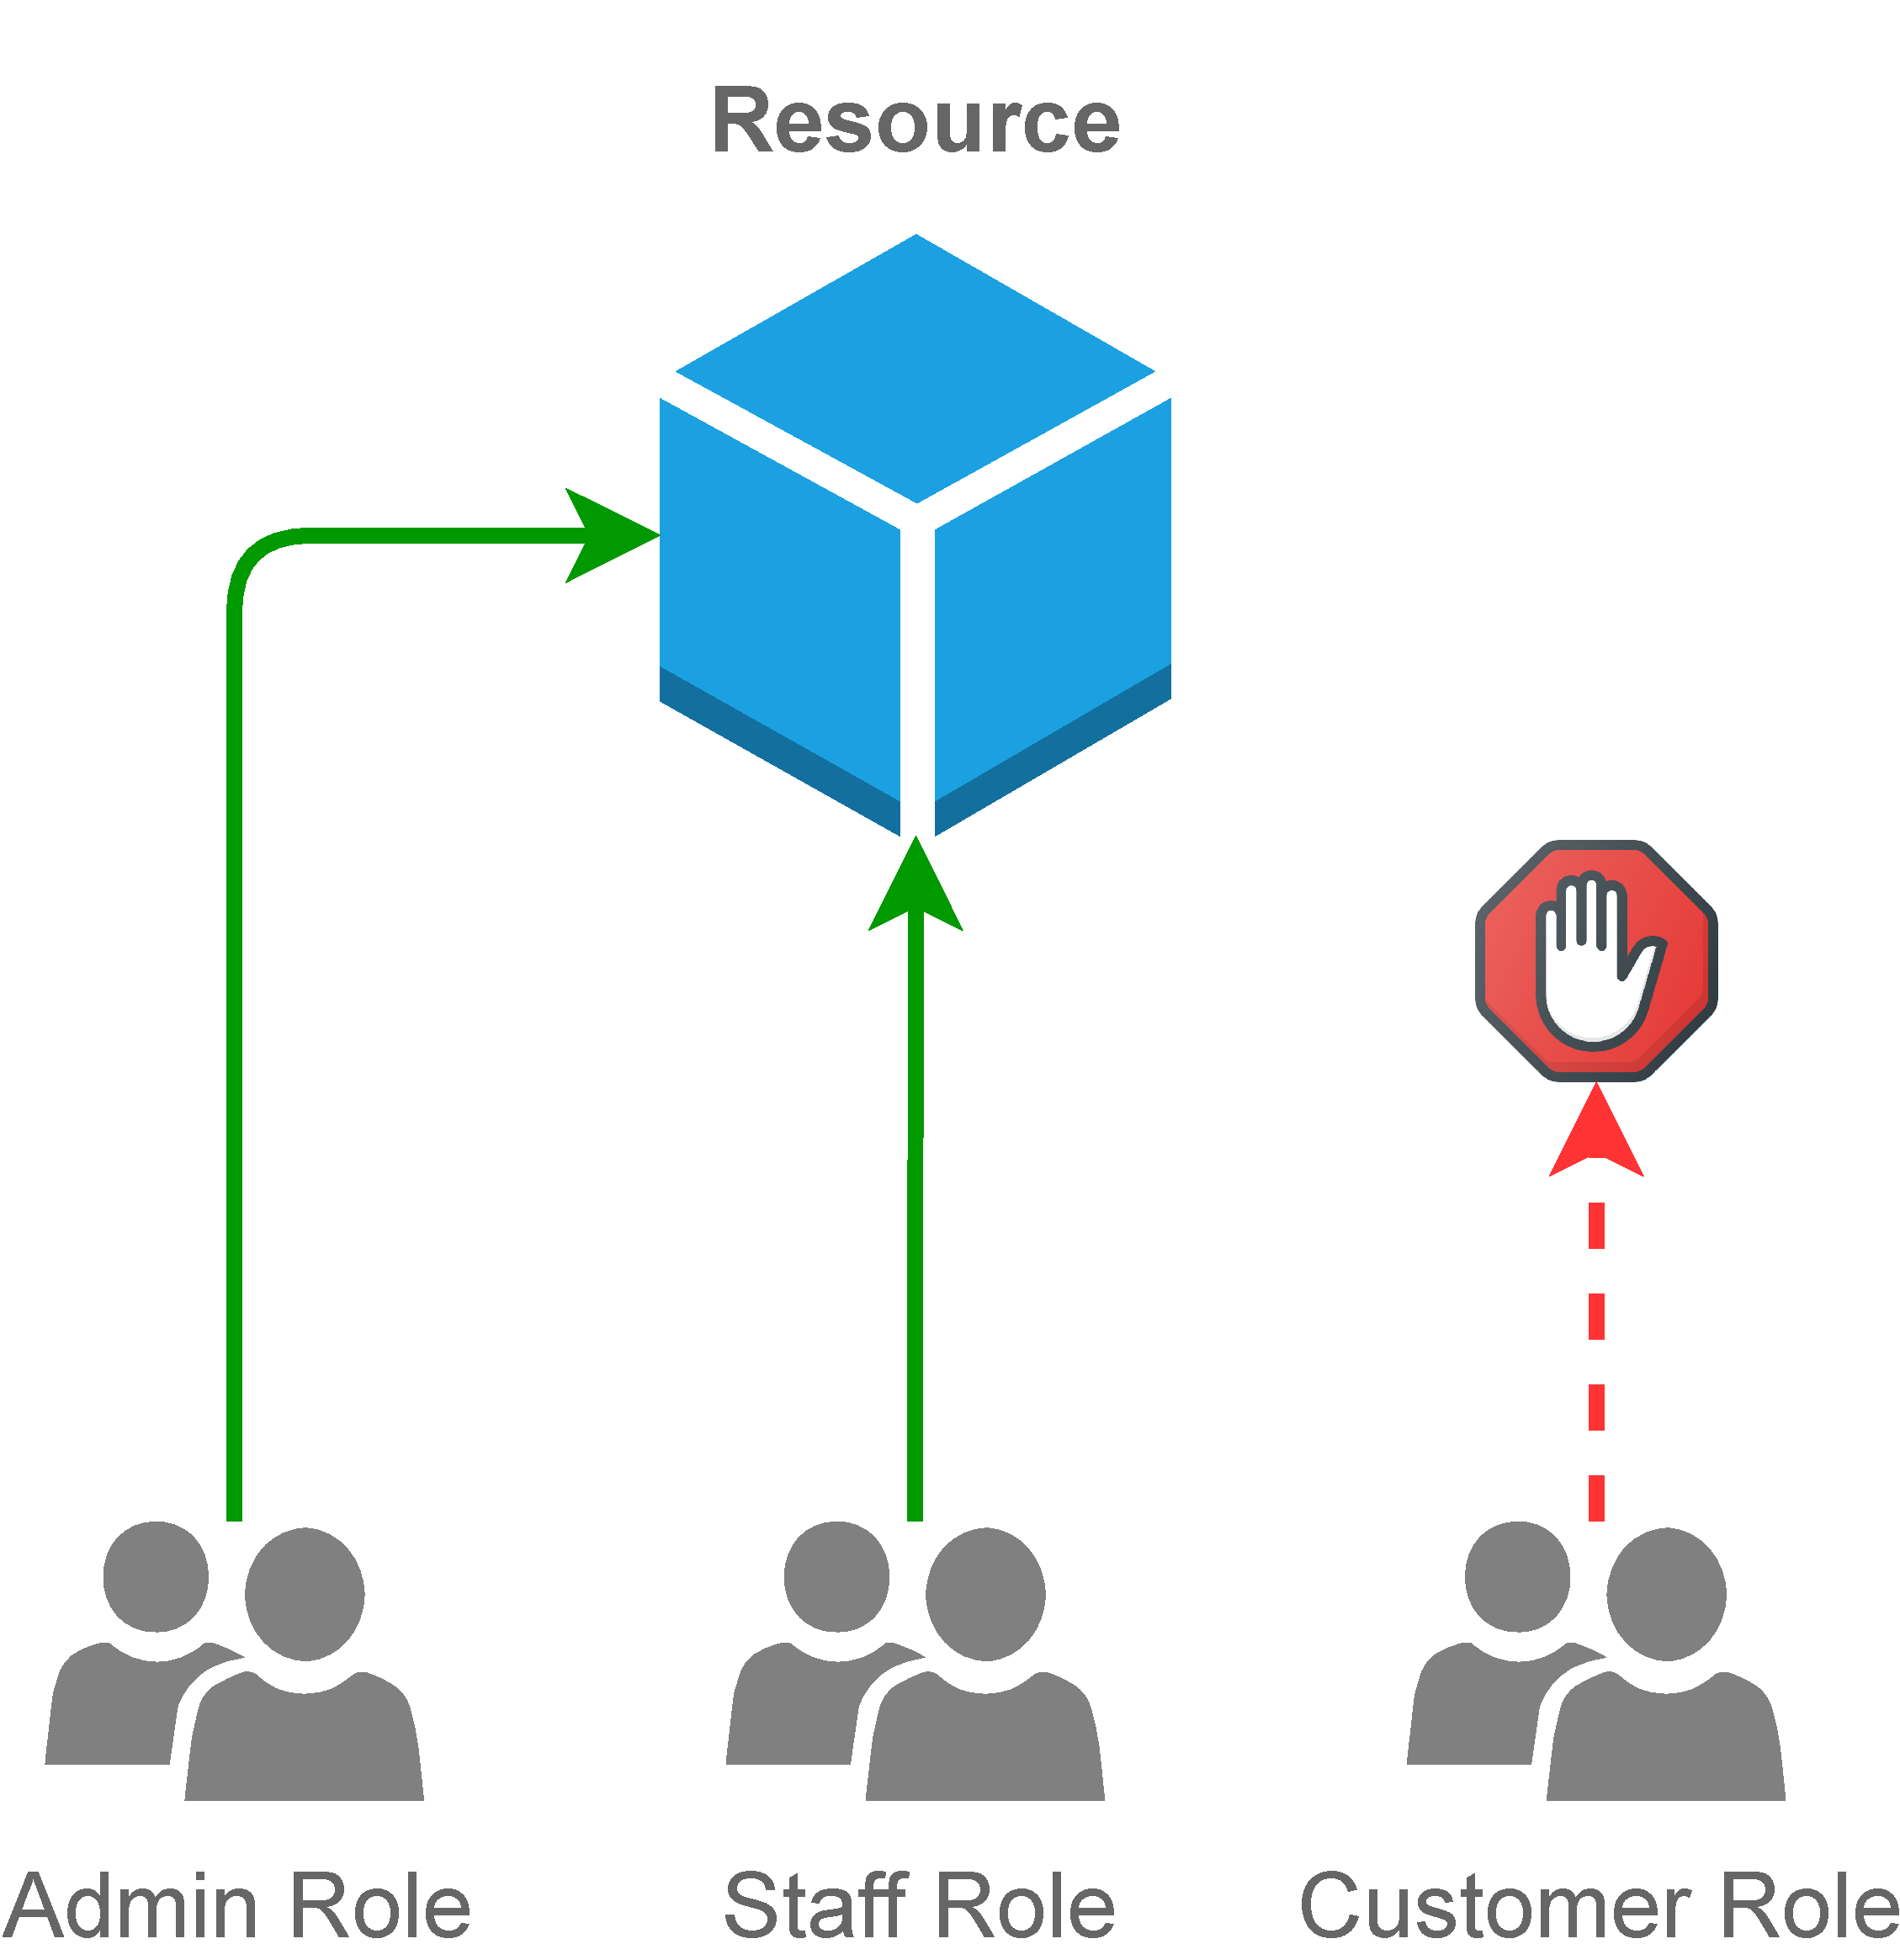
\includegraphics[width=0.65\linewidth]{images/chap5/RBCA.pdf}
    \caption{Illustration of resource access in the system according to the user's role type, following the \acrfull{rbac} model.}
    \label{fig:RBAC}
\end{figure}

Therefore, by adopting measures such as Role-Based Access Control (RBAC), the system effectively ensures the security and integrity of data. This is achieved by limiting and regulating access to system resources based on user roles. As a result, only authorized users can interact with relevant data and perform permitted actions. These restrictions not only strengthen the application's security but also contribute to maintaining data integrity.

\subsubsection{Authentication}

In addition, a security system based on access tokens has been implemented, utilizing JWT encoding\footnote{The JSON Web Token (JWT) is an advanced construct embedded within a JSON object, carefully defined according to the specifications of RFC 7519 \cite{johns_2016}. It serves as a secure channel for the transfer of a collection of information between two distinct parties. This mechanism provides a solid method for data transmission, notable for its verifiability and reliability, attributes that arise from its inherent ability to be digitally signed \cite{Ahmed9022766}.}. This encoding system is more flexible than using session cookies, as the process of verifying access permissions to resources with JWT is much simpler and comprehensive. The server does not need to make frequent queries to the database or store additional session information since all the necessary information is contained within the token.


\subsection{Assessment of System Capacity to Retrieve Project Information}

Having the ability to receive updates on the progress of a specific project and share relevant information about it is extremely important for project management \cite{lamptey2012developing}. This capability allows for tracking the project's progress and ensuring that all involved parties are aligned. Additionally, sharing media information such as images and documents related to the project aids in effective communication among teams and knowledge sharing \cite{Ihab}. Thus, this section aims to evaluate the system's ability to provide such data.

\subsubsection{Resources Served}
In order to assess the capability of the developed architecture in providing the necessary data, the code responsible for this functionality was made available, which can be found in Appendix \ref{apendice2} under the name of \href{https://github.com/iaggocapitanio1/woodWork4.0_API}{WW4 API}, along with the corresponding endpoints and services. Furthermore, a real visualization of the shared data was created in the web application, making the concepts more tangible and understandable. This direct approach allows for checking how the architecture is able to provide the data and how it is presented in the application's interface. This concrete demonstration aids in evaluating the architecture's capability and validating the established requirements.

For instance, Table \ref{tab:backend_resources} presents a list of resources provided by the developed system. The first column provides a brief summary of the resource's address, the second column contains the URL pointing to the corresponding service, and the third column briefly describes what each resource represents.

\begin{table}[!h]
\centering
\begin{tabular}{l l l }
\hline
\textbf{Name} & \textbf{URL Address} & \textbf{Description} \\
\hline
Address & \href{http://193.136.195.25/ww4/api/v1/accounts/address/}{/api/v1/accounts/address/} & User's adresses\\
Assembly & \href{http://193.136.195.25/ww4/api/v1/assembly/}{/api/v1/assembly/} & Projects's assembly \\
Auth Token & \href{http://193.136.195.25/ww4/auth/token}{/auth/token} &  Authentication Token\\
Budget & \href{http://193.136.195.25/ww4/api/v1/budget/}{/api/v1/budget/} & Project's budget \\
Consumable & \href{http://193.136.195.25/ww4/api/v1/consumable/}{/api/v1/consumable/} & Project's consumable \\
Customer Auth & \href{http://193.136.195.25/ww4/api/v1/accounts/customer/}{/api/v1/accounts/customer/} & WW4 Auth customer \\
Email  & \href{http://193.136.195.25/ww4/api/v1/email/service/}{/api/v1/email/service/} & Email service \\
Expedition & \href{http://193.136.195.25/ww4/api/v1/expedition/}{/api/v1/expedition/} & Project's expedition\\
Files & \href{http://193.136.195.25/ww4/api/v1/storages/file/}{/api/v1/storages/file/} & Projects's files \\
Folders & \href{http://193.136.195.25/ww4/api/v1/storages/folder/}{/api/v1/storages/folder/} & Projects's folders \\
Furniture & \href{http://193.136.195.25/ww4/api/v1/furniture/}{/api/v1/furniture/} & Projects's furnitures \\
Group & \href{http://193.136.195.25/ww4/api/v1/group/}{/api/v1/group/} & Projects's packaging\\
Groups  & \href{http://193.136.195.25/ww4/api/v1/perms/group/}{/api/v1/perms/group/} & Group permissions \\
Invalidate Sessions & \href{http://193.136.195.25/ww4/auth/invalidate-sessions}{/auth/invalidate-sessions} & Invalidate Session Cookie \\
Invalidate Token & \href{http://193.136.195.25/ww4/auth/revoke-token}{/auth/revoke-token} &  Invalidate JWT token \\
Leftover & \href{http://193.136.195.25/ww4/api/v1/leftover/}{/api/v1/leftover/} & Leftover entity \\
Leftover Image & \href{http://193.136.195.25/ww4/api/v1/storages/leftover/}{/api/v1/storages/leftover/} & Leftover images\\
Machine & \href{http://193.136.195.25/ww4/api/v1/machine/}{/api/v1/machine/} &  Organization's machines \\
Messages & \href{http://193.136.195.25/ww4/api/v1/chat/message/}{/api/v1/chat/message/} & Message service \\
Module & \href{http://193.136.195.25/ww4/api/v1/module/}{/api/v1/module/} & Project's module\\
Organization & \href{http://193.136.195.25/ww4/api/v1/accounts/organization/}{/api/v1/accounts/organization/} & WW4 Auth Organization \\
Owner & \href{http://193.136.195.25/ww4/api/v1/owner/}{/api/v1/owner/} & Project's owner \\
Permissions & \href{http://193.136.195.25/ww4/api/v1/perms/permission/}{/api/v1/perms/permission/} & Avaliable permissions \\
Part & \href{http://193.136.195.25/ww4/api/v1/part/}{/api/v1/part/} & Project's parts \\
Project & \href{http://193.136.195.25/ww4/api/v1/project/}{/api/v1/project/} & Project\\
Resend Activation & \href{http://193.136.195.25/ww4/api/v1/accounts/reactivate}{/api/v1/accounts/reactivate} & Token to activate account\\
Reset Password & \href{http://193.136.195.25/ww4/api/v1/accounts/reset-password}{/api/v1/accounts/reset-password} & Token to activate password \\
Tag & \href{http://193.136.195.25/ww4/api/v1/tag/}{/api/v1/tag/} & Upload tags \\
Tag Result & \href{http://193.136.195.25/ww4/api/v1/tag-result/}{/api/v1/tag-result/} & Corrected Tags \\
Worker & \href{http://193.136.195.25/ww4/api/v1/worker/}{/api/v1/worker/} & WW4 Auth Worker \\
Worker-task & \href{http://193.136.195.25/ww4/api/v1/worker-task/}{/api/v1/worker-task/} & Bridge table for worker and part \\
\hline
\end{tabular}
\caption{List of resources provided by the backend service}
\label{tab:backend_resources}
\end{table}

 This \gls{api} embeds all the necessary URLs, enabling the User Interface to efficiently consume the information. The figure presents a visual representation of the different URLs available in the API, highlighting the connectivity between the endpoints and the interaction with the user interface. This provides a clear view of how data is accessed and used by the application.


To elucidate the results more concretely, it was decided to demonstrate the performance of the Web interface using images. This interface, which feeds on the information provided by the \gls{api}, provides a more tangible view of the system's operation. Figures \ref{fig:results-dash1} and \ref{fig:results-dash3} represent data from the \gls{api} being consumed, thus illustrating the traceability of project information.

\begin{figure}[H]
    \centering
    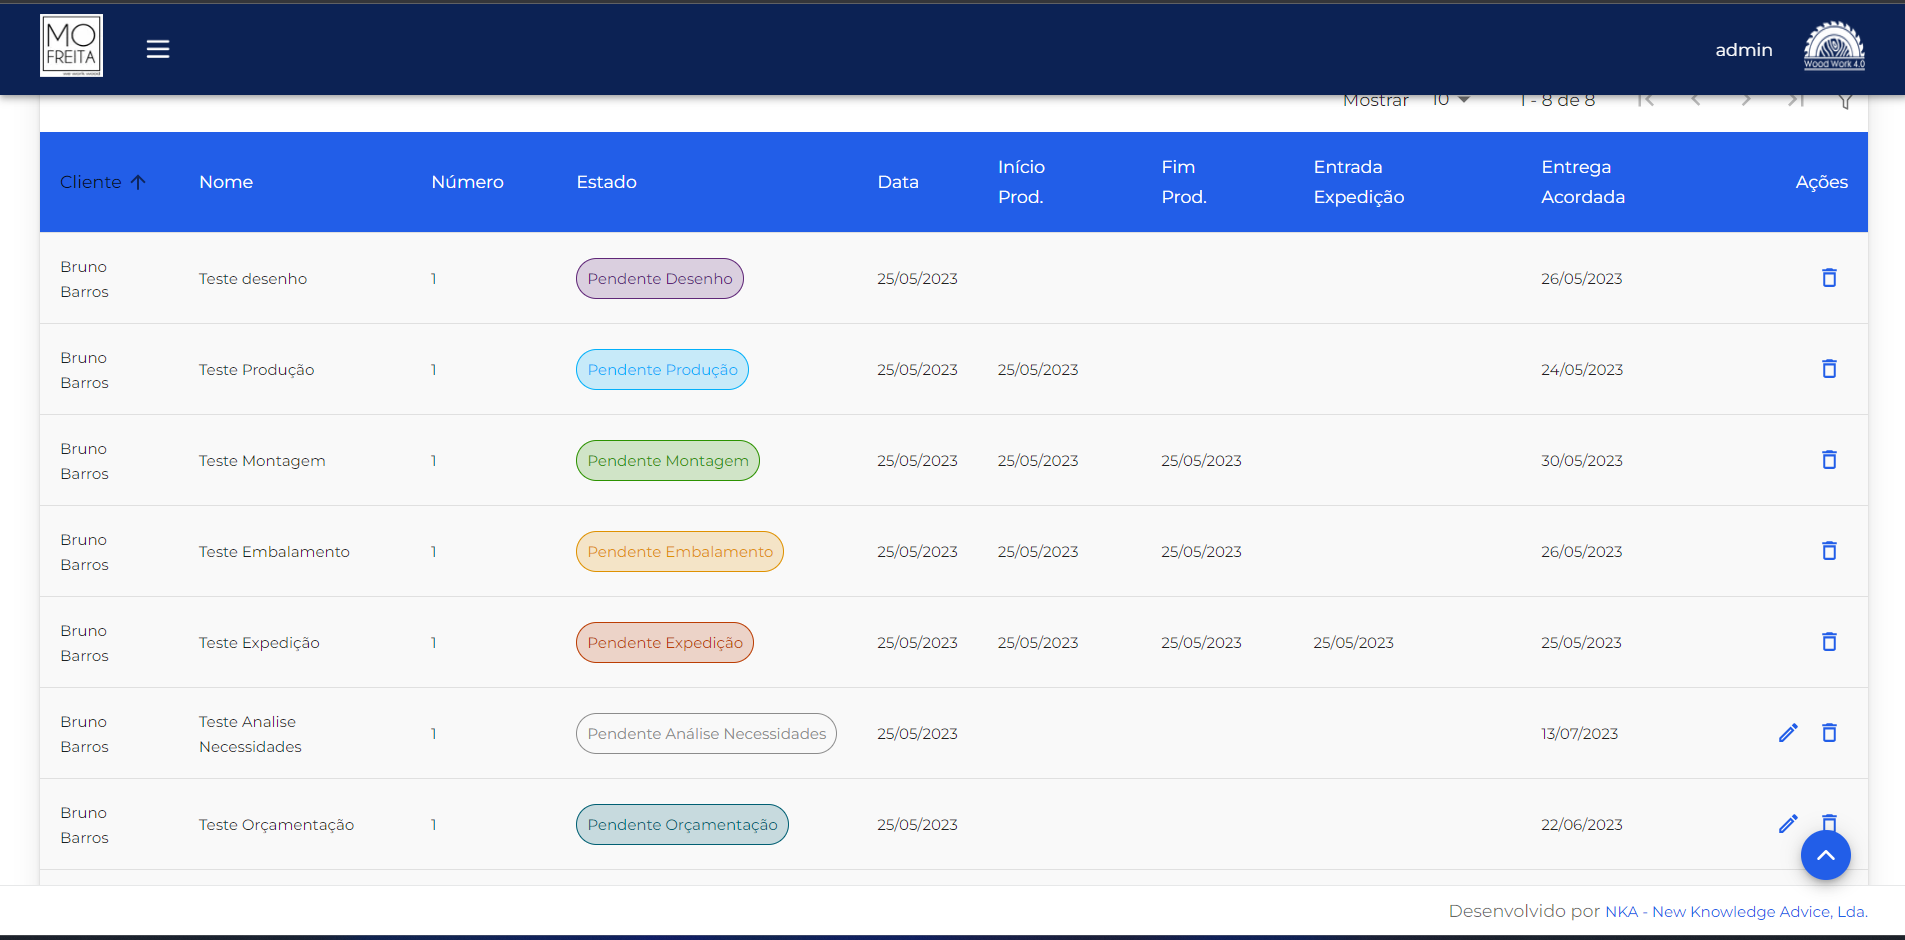
\includegraphics[width=0.65\linewidth]{images/chap5/dashboard02.png}
    \caption{Project status dashboard: a crucial asset for holistic project monitoring and customer order tracking and project management.}
    \label{fig:results-dash1}
\end{figure}


\begin{figure}[!ht]
    \centering
    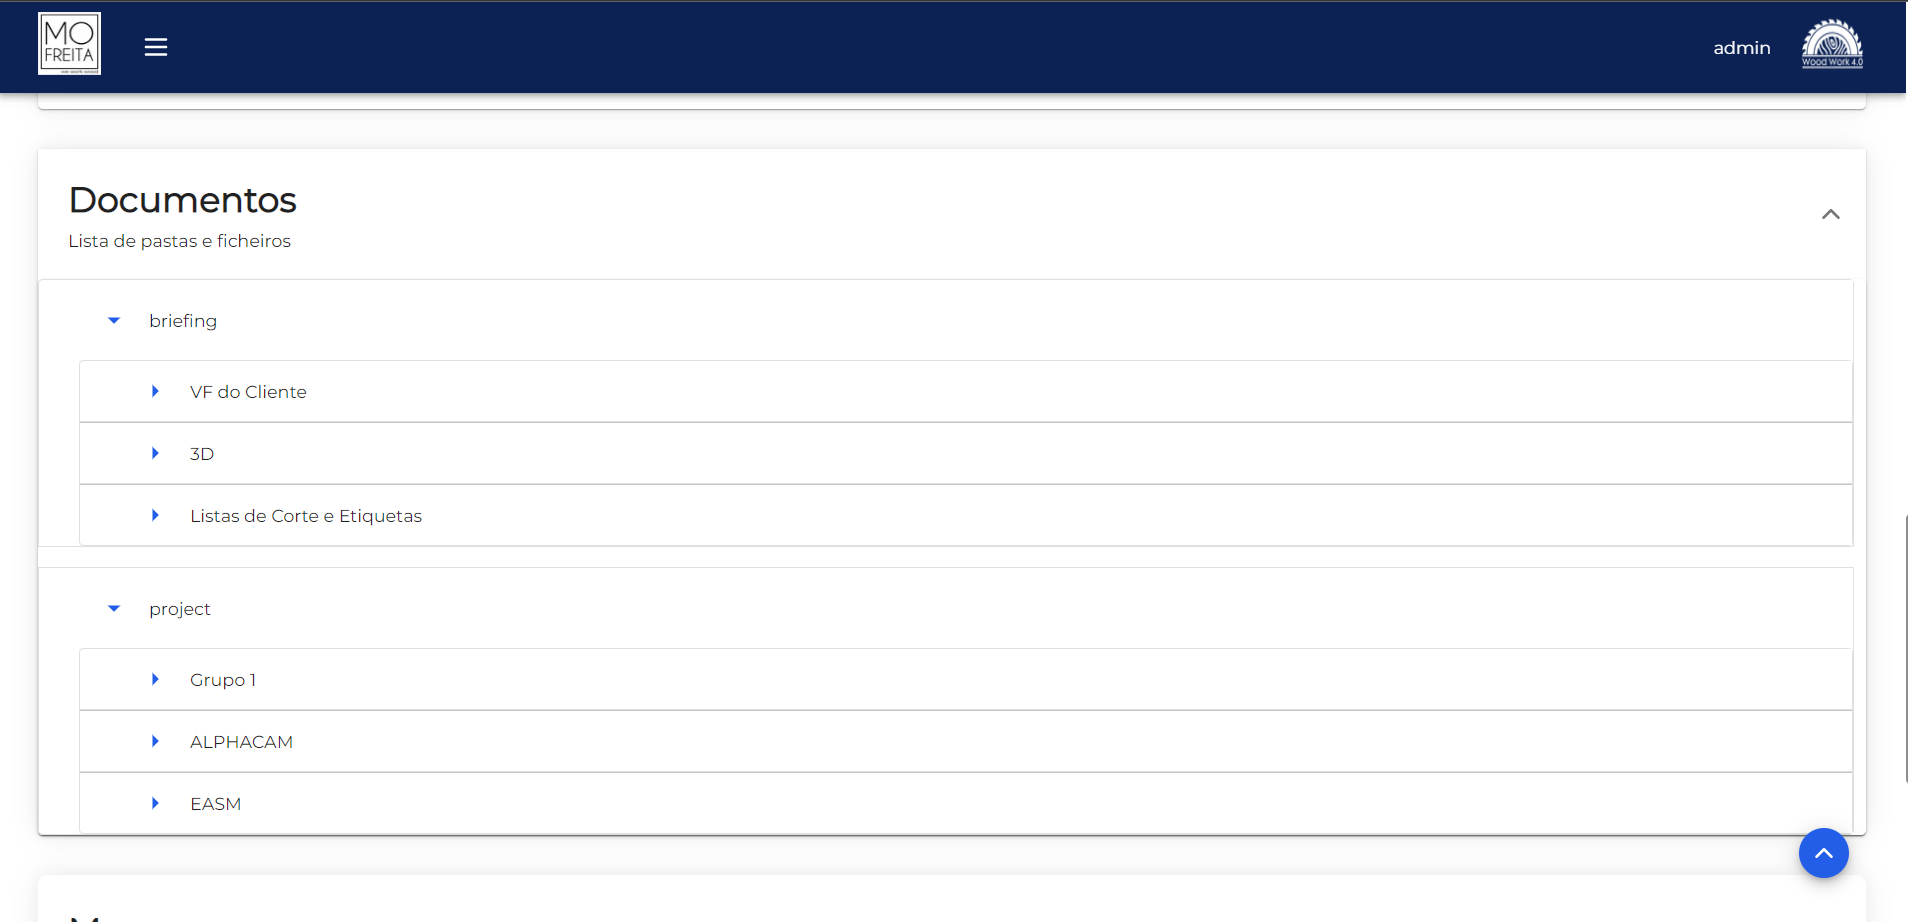
\includegraphics[width=0.65\linewidth]{images/chap5/dashboard03.png}
    \caption{Web interface displaying the capability to share media data stored on the Mofreitas server. The interface showcases the mirrored folders on the server, allowing users to access and share media files.}
    \label{fig:results-dash3}
\end{figure}


\subsection{Overview of the Developed Architecture}

The architecture developed in this work encompasses various essential components for an efficient and secure information management system. This architecture integrates several security measures previously discussed, along with a system for file sharing and project information management. Such integration enables not only the traceability of a project as a whole but also that of individual elements, such as leftovers.

One of the  aspects of the architecture is the incorporation of a communication system, which includes message sharing and an email service. Moreover, an authentication module ensures that only authorized users have access to relevant information. Notably, the architecture capitalizes on advancements in the field of computer vision for text recognition, which significantly contributes to the correction of some tags utilized in the manufacturing process. Additionally, the architecture is capable of logging the history of various transactions, providing a robust data-set . This tracking capability and transaction history storage open doors for the application of big data analysis and machine learning algorithms. Such application can enable continuous system optimization and yield valuable insights, which can contribute to more informed decision-making.

Finally, the combination of integrated technologies and the ability to adapt and evolve with new trends and demands, brings the system closer to the concept of a smart product. It stands out for its interoperability, scalability, and harmonious integration with multiple technologies, creating a comprehensive solution that meets the dynamic and complex needs of information management in a production environment.

\begin{figure}[!ht]
    \centering
    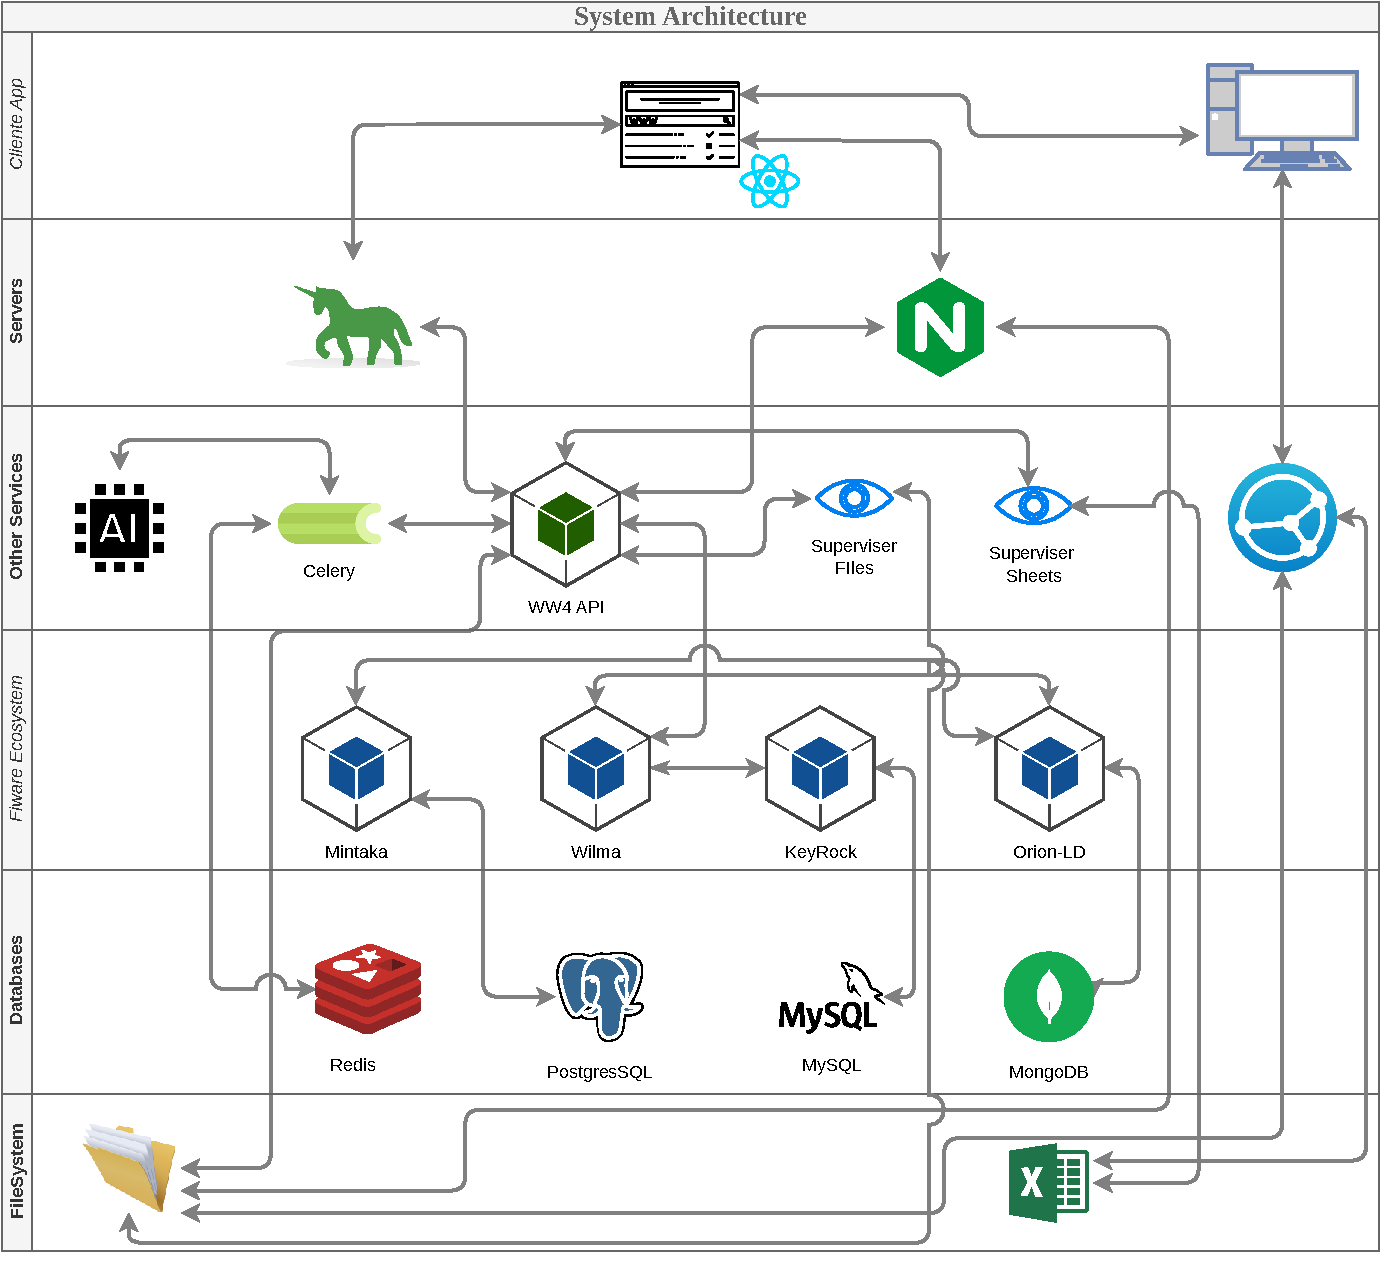
\includegraphics[width=0.75\linewidth]{images/chap5/Arch.pdf}
    \caption{Overview of the Developed Architecture.}
    \label{fig:arch-overview}
\end{figure}

\section{Ability of the System to Detect Leftovers}

The ability of the system to detect leftovers will depend on two essential factors. First, the system's ability to use image processing to accurately and efficiently identify leftovers. This involves the use of algorithms and computer vision techniques to analyze the images and identify the desired objects. Second, the system's ability to read and send relevant information to the company's database. After detecting the leftovers, it is important that the system is able to extract the necessary data and send it to the company's central database. This allows for the storage and subsequent analysis of the collected information, enabling appropriate decision-making.

\subsection{Measurement System}

The developed measurement system consists of an embedded processing unit together with a camera, as detailed in section \ref{section:embeddedSystem}. In this system, data is captured by the camera and undergoes a processing process before being sent to the Mofreitas company's server. The assembly of the system at Mofreitas can be seen in Figures \ref{fig:montagem2} and \ref{fig:camera2}.

\begin{figure}[!h]
    \centering
    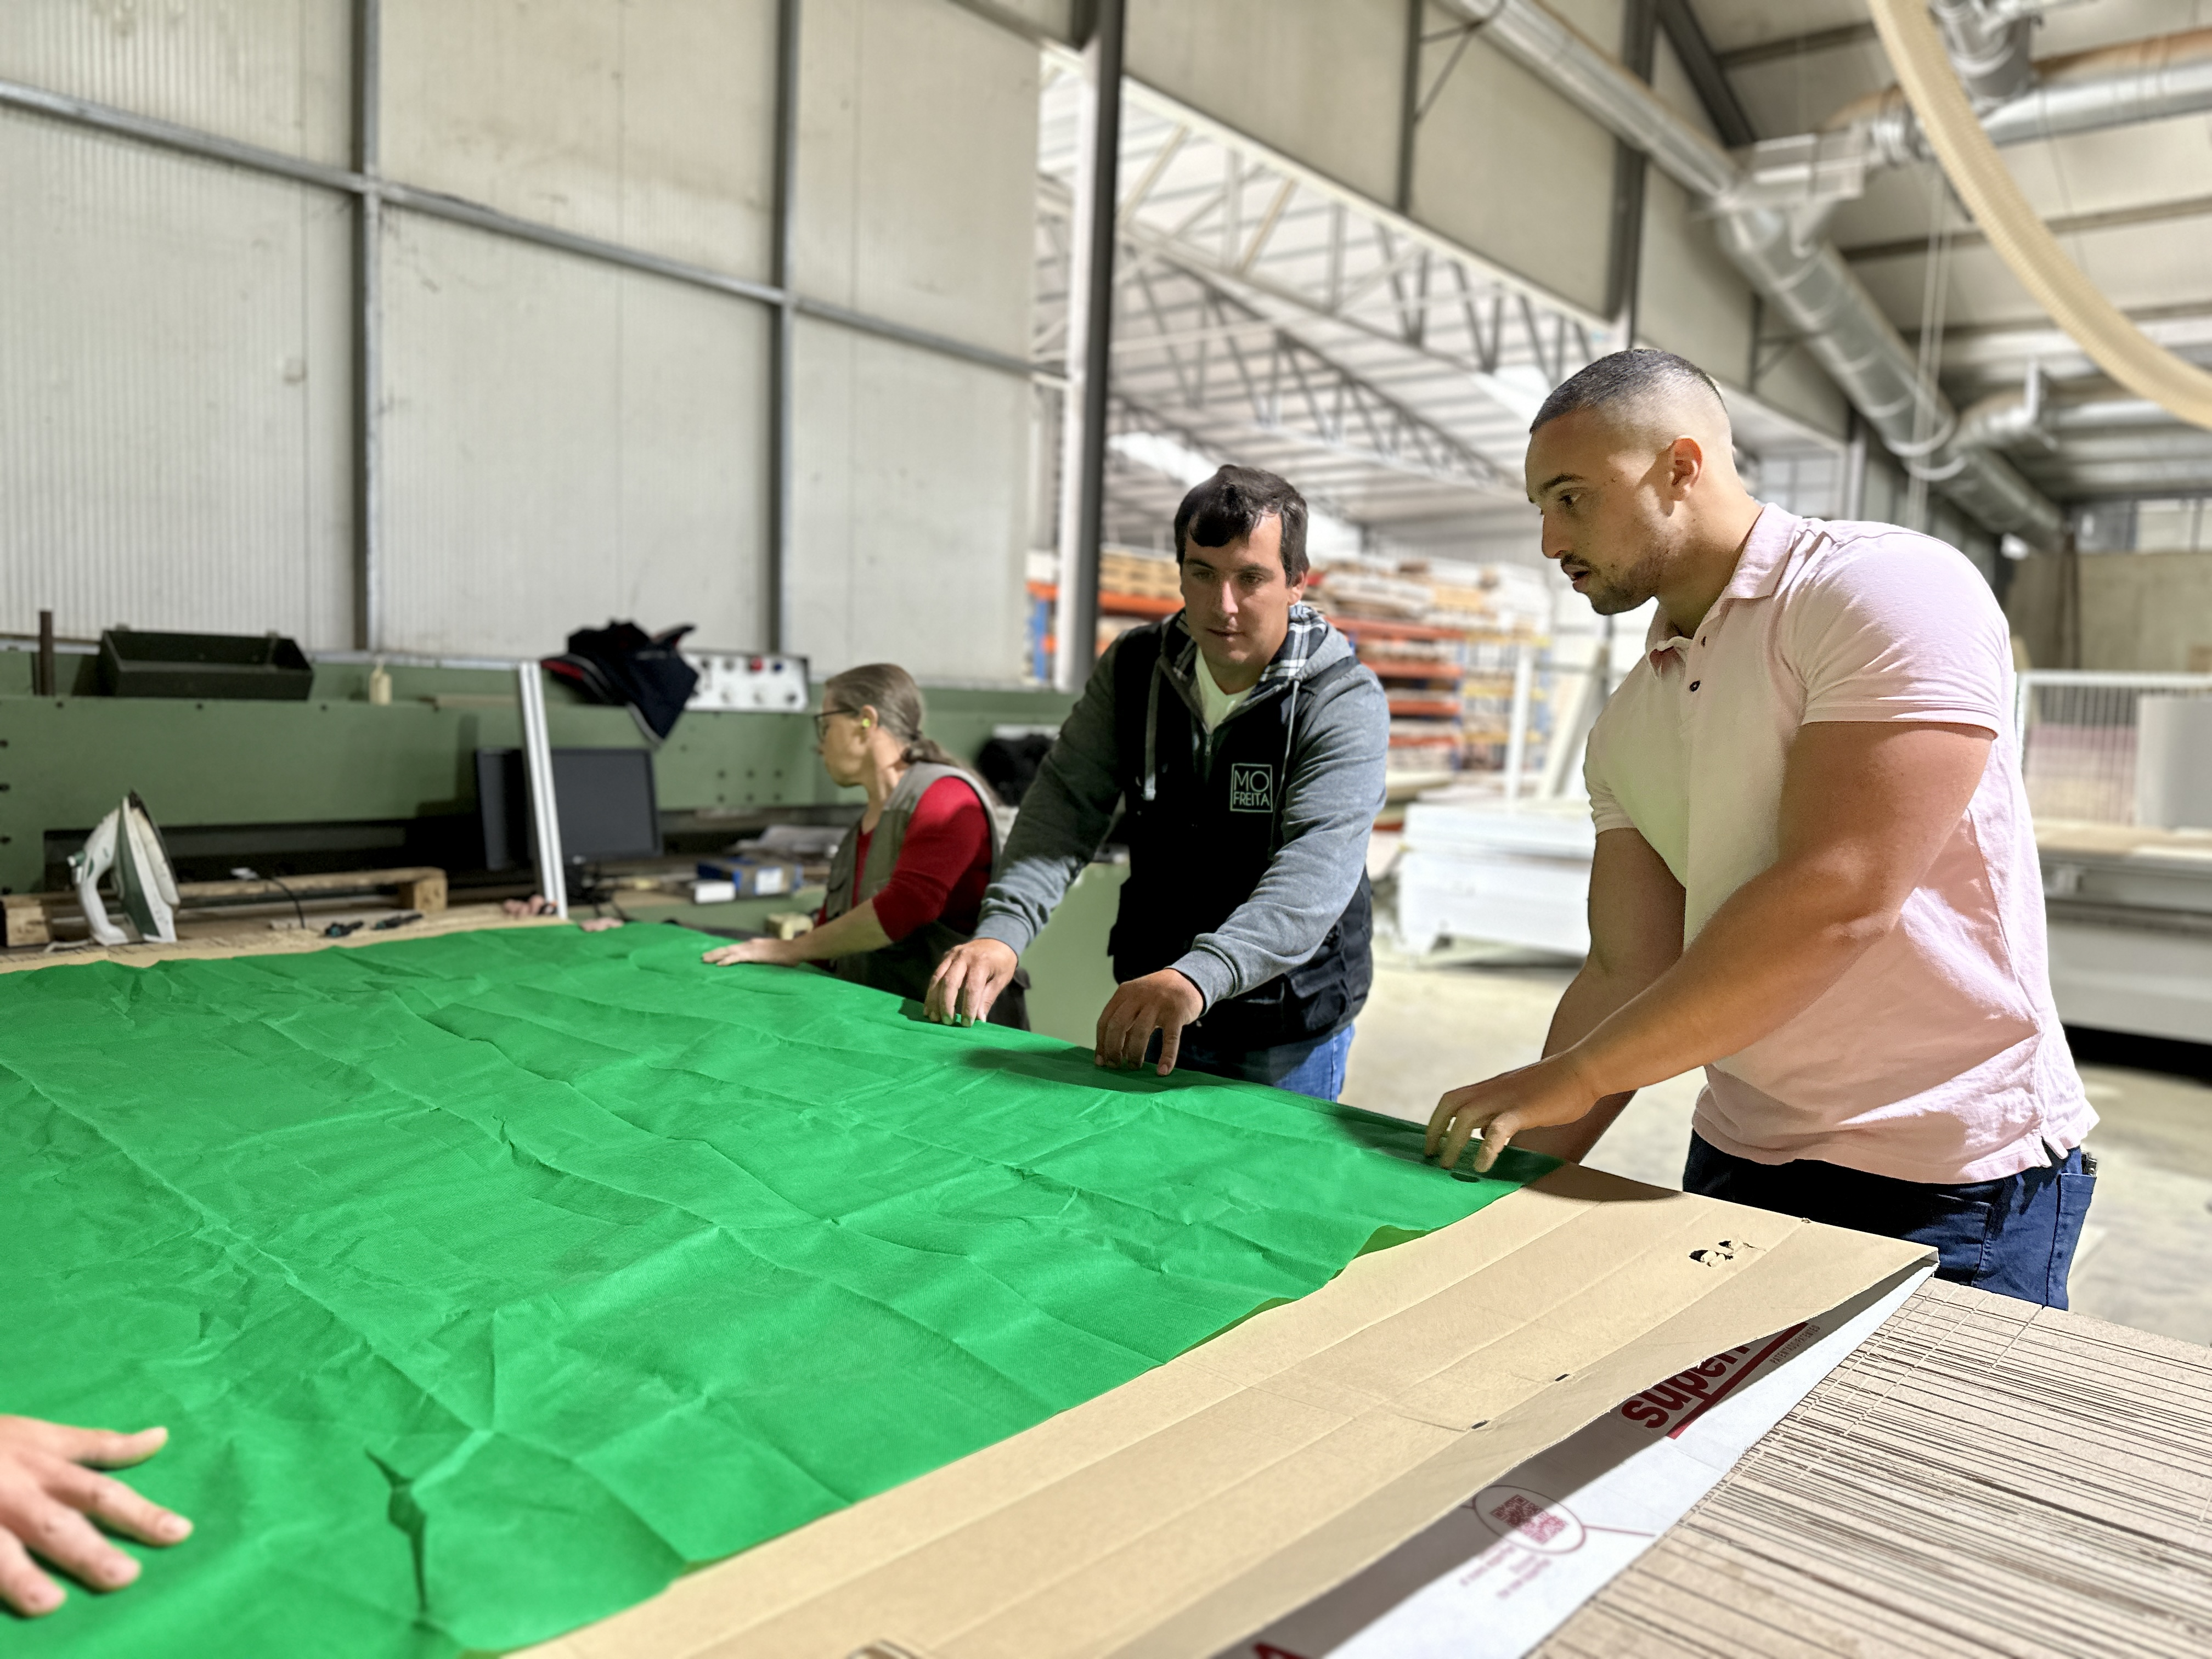
\includegraphics[width=0.55\linewidth]{images/chap5/montagem2.jpg}
    \caption{Preparation of the platform for leftovers measurement.}
    \label{fig:montagem2}
\end{figure}

\begin{figure}[!ht]
    \centering
    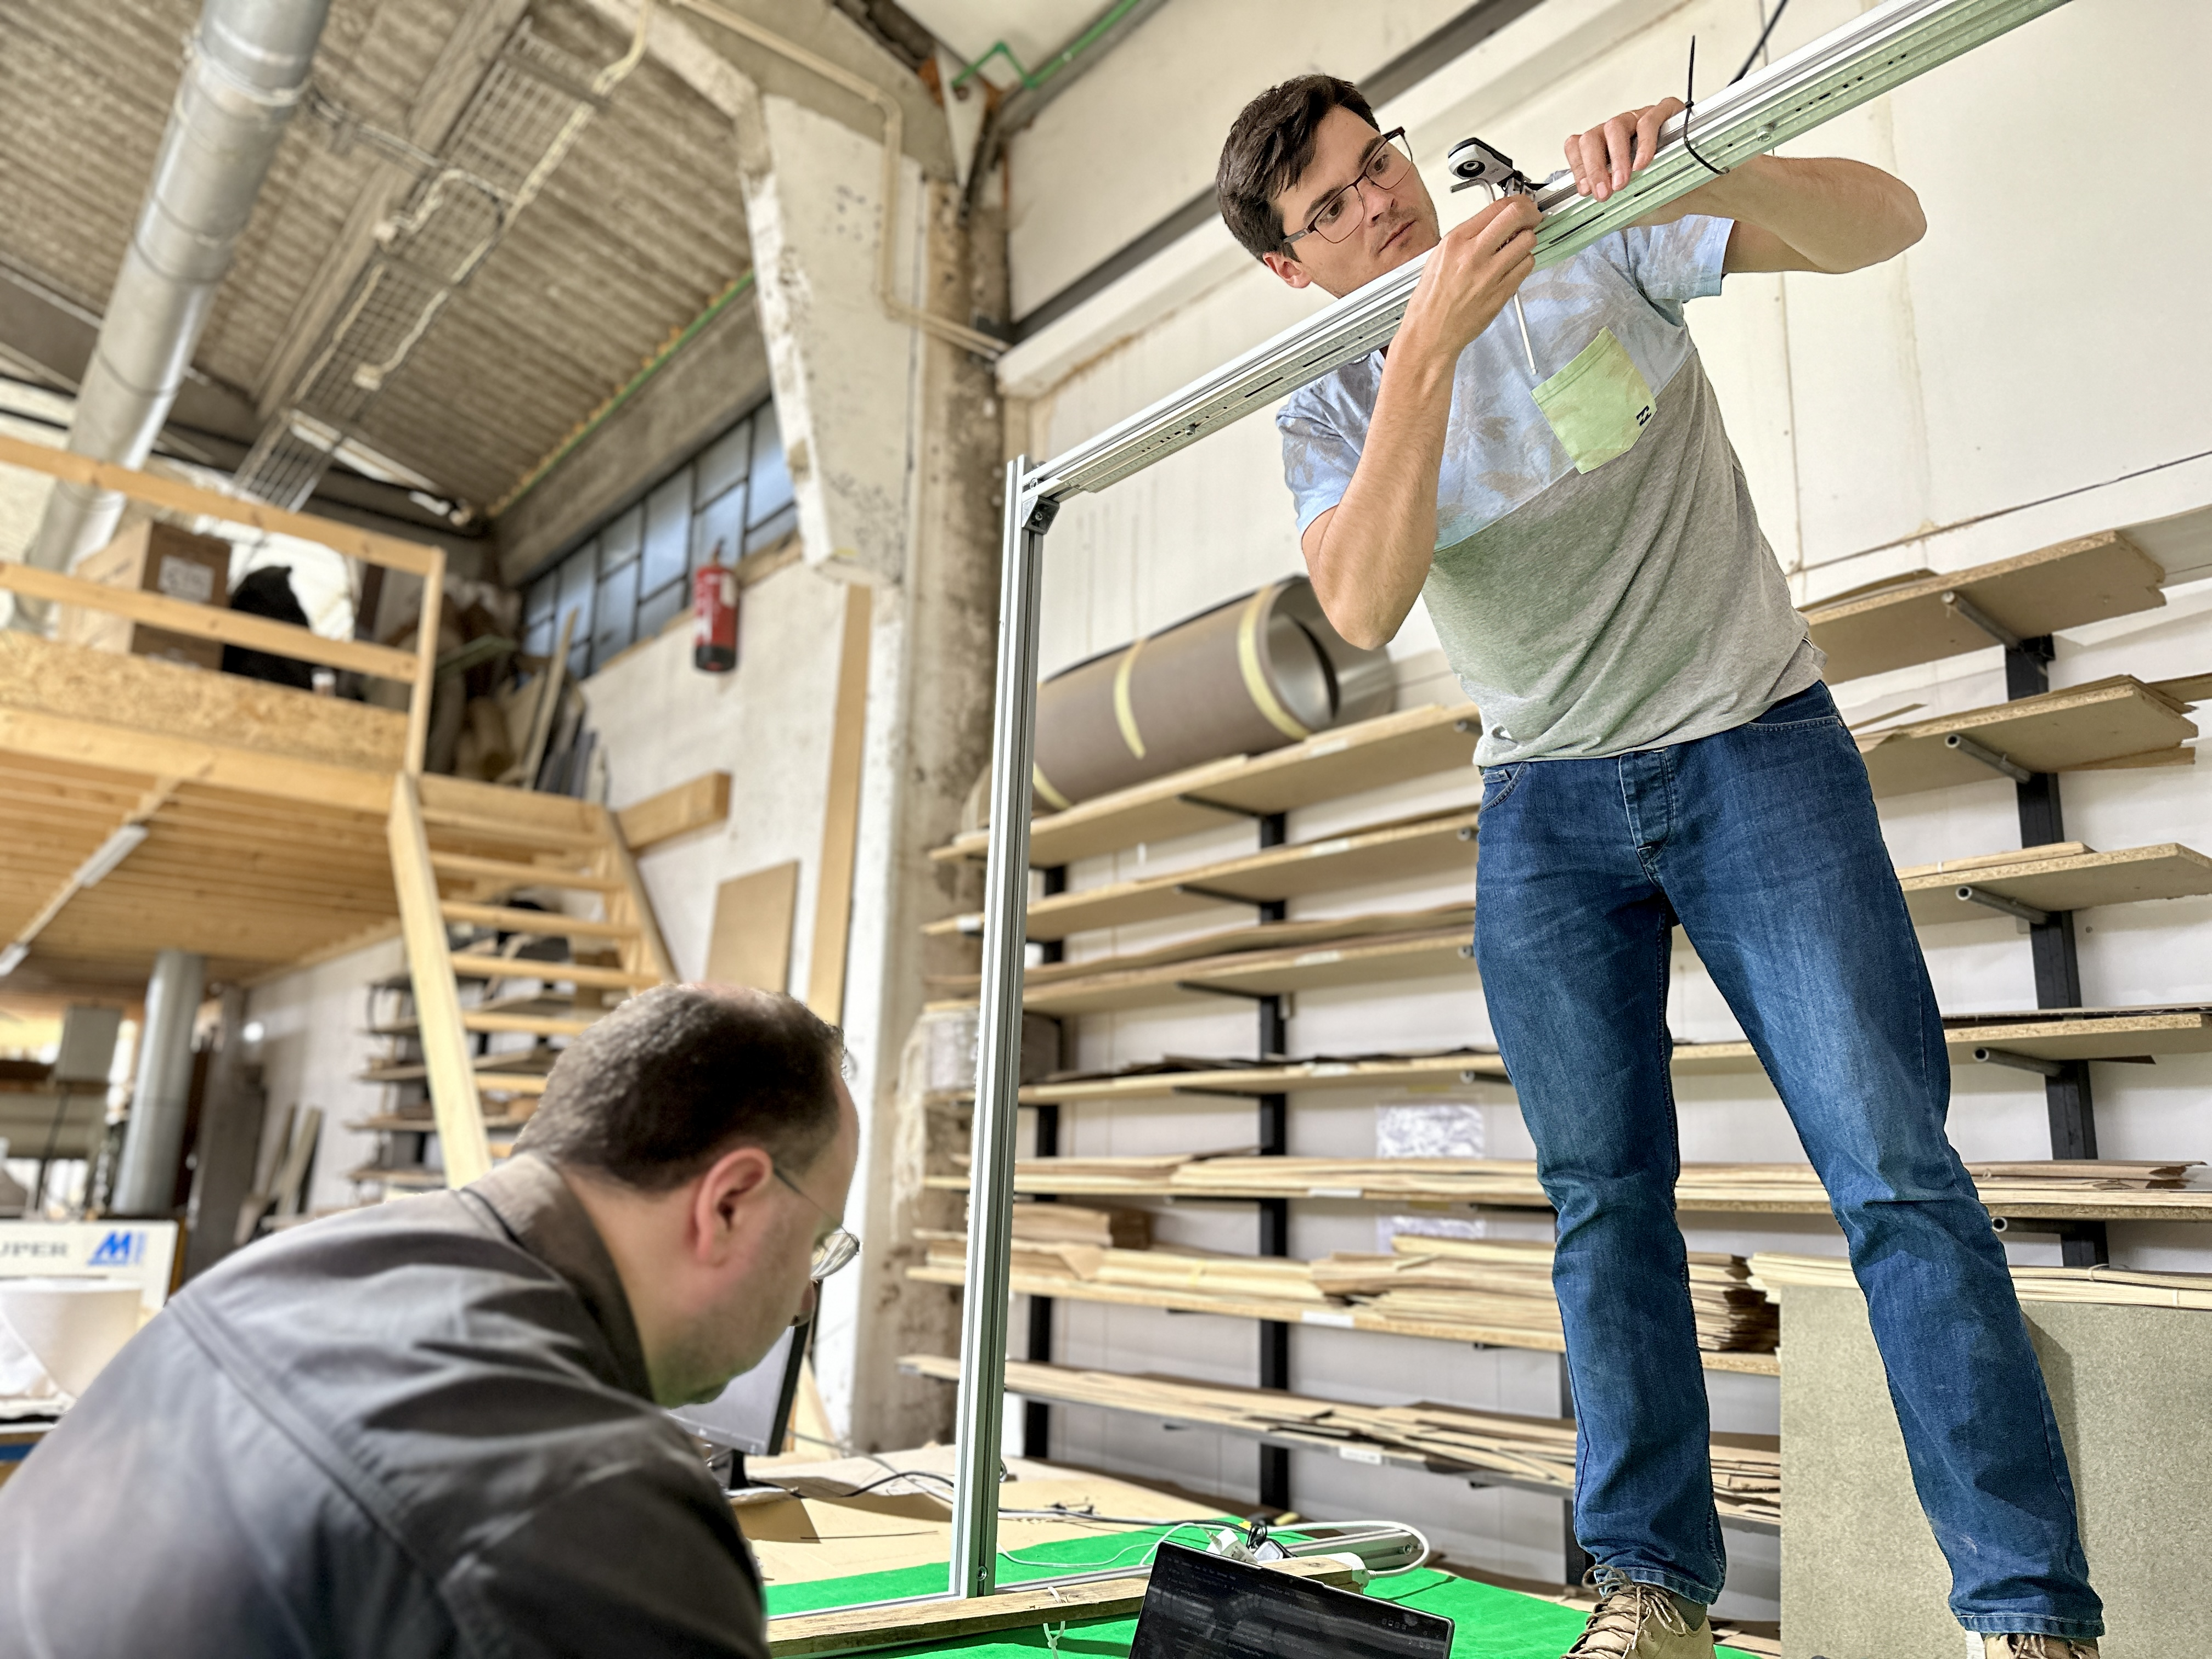
\includegraphics[width=0.55\linewidth]{images/chap5/camera2.jpg}
    \caption{Installation of the system for leftover detection, the photo shows the setup of the IDS camera.}
    \label{fig:camera2}
\end{figure}

The result of the processing can be observed in the following figure \ref{fig:imagemprocessing}.

\begin{figure}
    \centering
    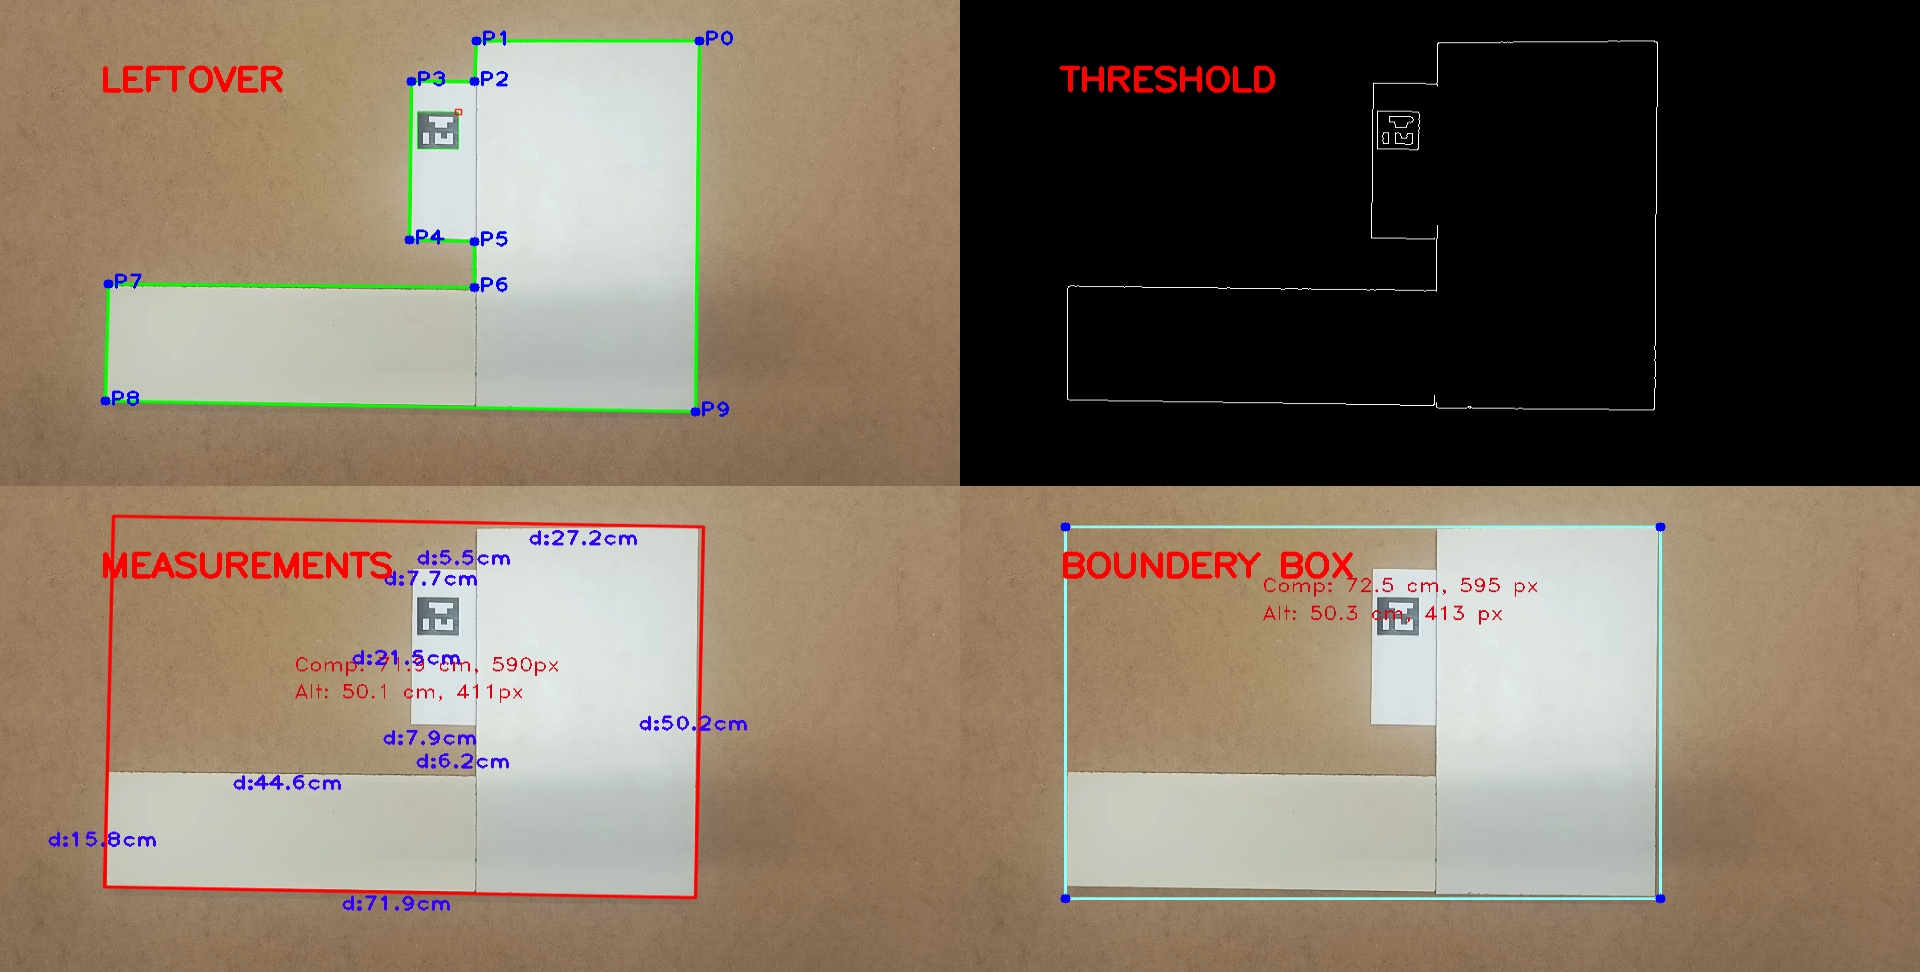
\includegraphics[width=0.65\linewidth]{images/chap5/imageProcessing.png}
    \caption{Result obtained from image processing, the image shows the four main stages of the image processing.}
    \label{fig:imagemprocessing}
\end{figure}

\newpage
\subsection{Methodology for Evaluating the Measurement Capability of the System.}

In order to evaluate the system's ability to perform measurements, measurements were conducted using both a conventional tape measure and a camera. This approach allowed for comparison of the results obtained by both methods and determine if the developed measurement system would be a viable alternative to replace the currently used manual methodology. The reason behind this consideration is that the manual approach requires significant effort and faces implementation difficulties in a manufacturing environment. Therefore, this situation presents an opportunity for the implementation of the developed system.

In the experiment, measurements were taken with the camera positioned at a distance of 180 cm from the wooden pieces. As shown in Figure \ref{fig:methodology}, which illustrates the process.

\begin{figure}
    \centering
    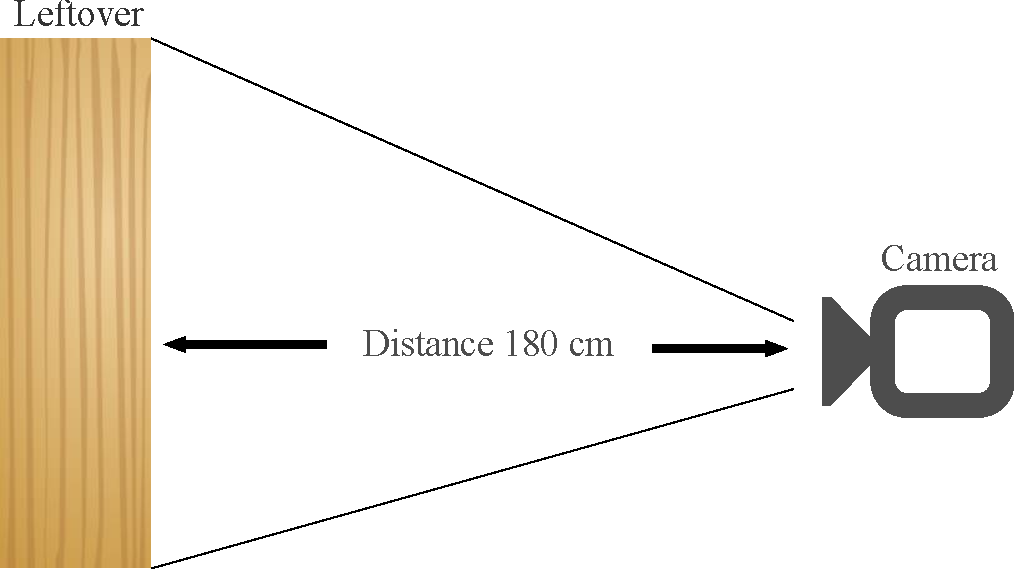
\includegraphics[width=0.65\linewidth]{images/method.pdf}
    \caption{Illustration of how the measurements were carried out for the evaluation of the measurement results. The chamber was placed at about 180 cm away from the leftovers.}
    \label{fig:methodology}
\end{figure}

The Table \ref{tab:leftovers} presents the data obtained during the measurement of a sample group of twelve pieces. The images used for data acquisition are available in Appendix \ref{apendice2}.

It's important to underline that the dimensions of a piece can vary; in other words, each side can exhibit different measurements. To achieve a precise average value of these dimensions, the strategy is to measure as close as possible to the center of each piece. This approach ensures that the approximations closely reflect the average dimensions of the piece. This method is employed for measurements taken with a tape measure.

For the image processing phase, the average of the values from parallel sides is considered. To illustrate, if the height on the left side of a piece is 5 cm and the corresponding height on the right side is 7 cm, the average of these two is taken as the definitive measurement. This procedure is depicted by the equation \eqref{eq:instance_h}.

\begin{equation}
    H = \frac{h_{left} + h_{right}}{2}
    \label{eq:instance_h}
\end{equation}

\begin{table}[h]
\centering

\begin{tabular}{c c c c}
\hline
\textbf{Ref Width} & \textbf{Measured Width} & \textbf{Ref Height} & \textbf{Measured Height} \\
\hline
 14.3 & 14.2 & 14.5 & 14.45 \\
 19.5 & 19.5 & 19.4 & 19.4 \\
47.5 & 47.55 & 13 & 12.85 \\
 20.5 & 20.5 & 20.3 & 20.15 \\
23.6 & 23.6 & 14.6 & 14.6 \\
24.5 & 24.35 & 10 & 9.95 \\
28.9 & 28.7 & 15.2 & 15.25 \\
 34.3 & 34.3 & 23.3 & 23.3 \\
42.5 & 42.35 & 6.2 & 6.4 \\
 43 & 42.85 & 14.9 & 14.65 \\
 47.5 & 47.55 & 13 & 12.85 \\
 48.1 & 48.2 & 21.7 & 21.75 \\
\hline
\end{tabular}
\caption{Width and Height Measurements}
\label{tab:leftovers}
\end{table}



The authors \textcite{bland1986statistical} developed a statistical methodology to assess the possibility of one type of measurement being used in place of another. The Bland-Altman method is a statistical technique used to evaluate agreement or difference between two measurement methods or assessment techniques. It involves calculating the differences between the measurements obtained by each pair of methods, creating a scatter plot of the differences against the mean of the measurements, and analyzing the agreement based on the dispersion of the points around the mean line and the limits of agreement lines. It is widely used in method comparison studies and instrument validation to assess agreement and identify systematic trends or bias. While an ideal model would state that the measurements would be exactly equal, there is always some degree of error in measurements. Even analytical imprecision generates variability in the differences \cite{giavarina2015understanding}. However, if the variability is related only to analytical imprecision, the mean of the differences would be zero. Therefore, the first step in assessing agreement is to observe the mean of the differences between the paired data.

\begin{figure}[!ht]
    \centering
    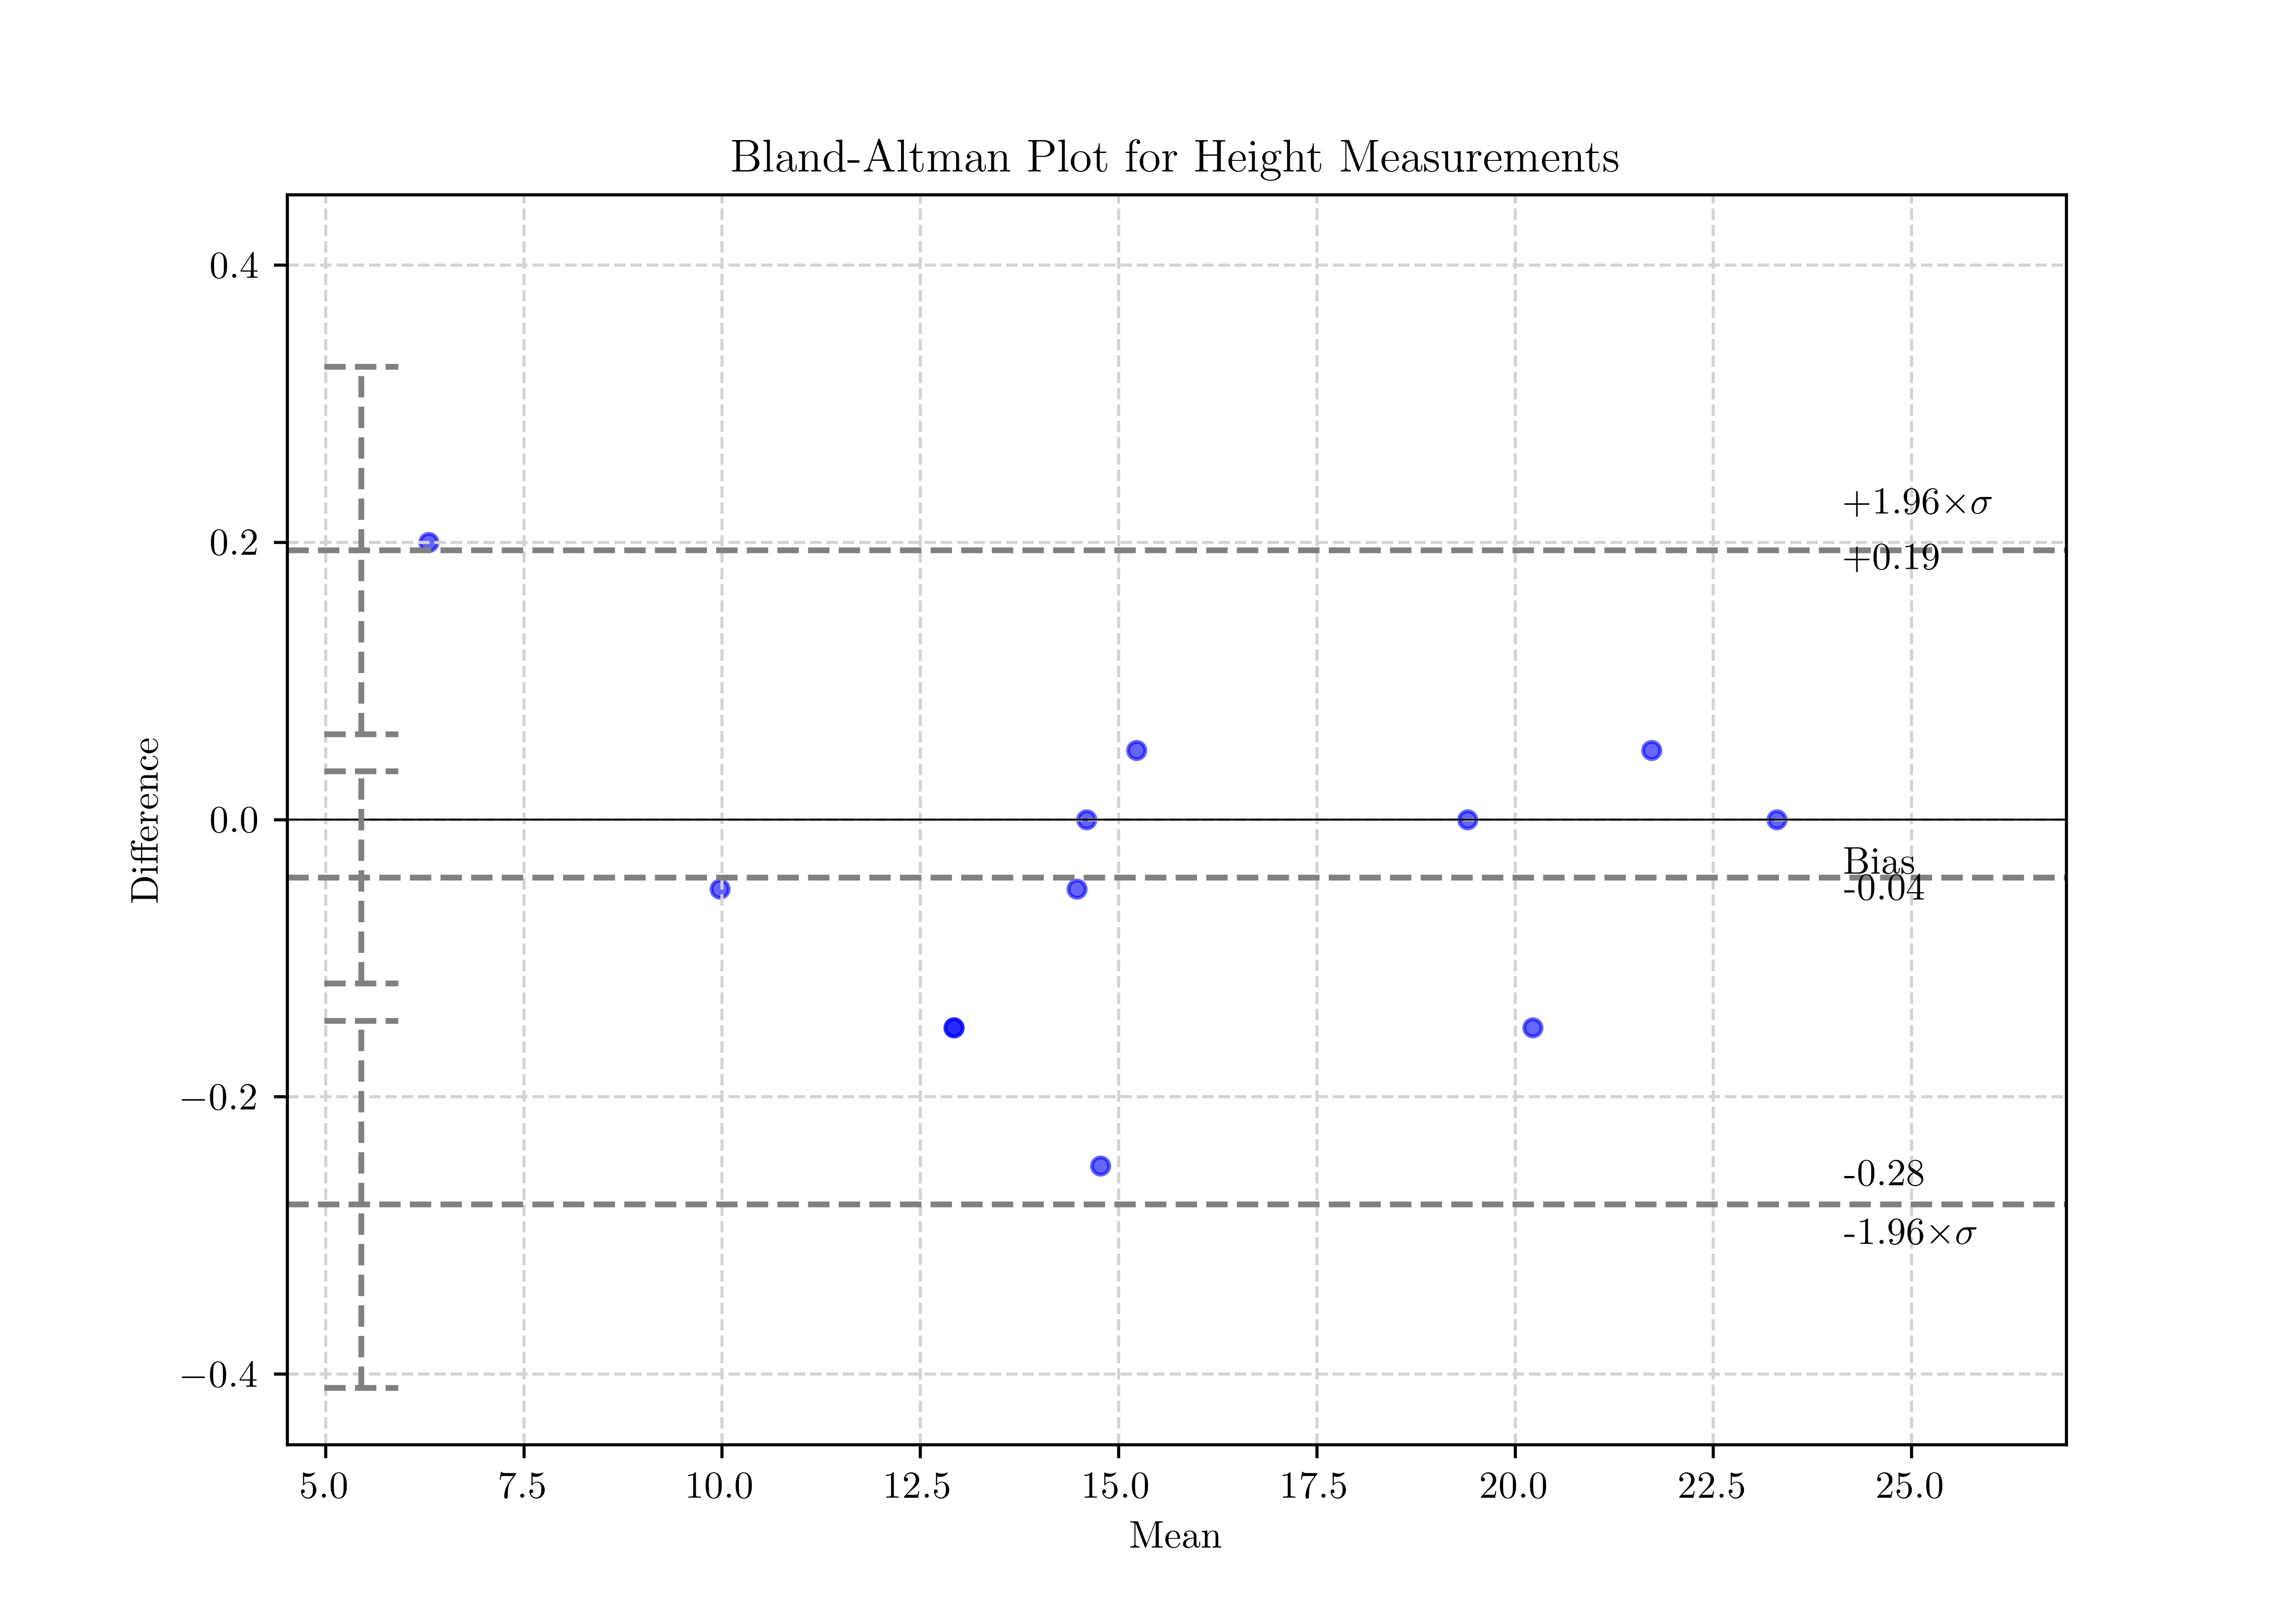
\includegraphics[width=0.75\linewidth]{images/chap5/height.png}
    \caption{Bland-Altman plot showcasing the height measurements obtained.}
    \label{fig:Bland-Altman_height}
\end{figure}

\begin{figure}[!ht]
    \centering
    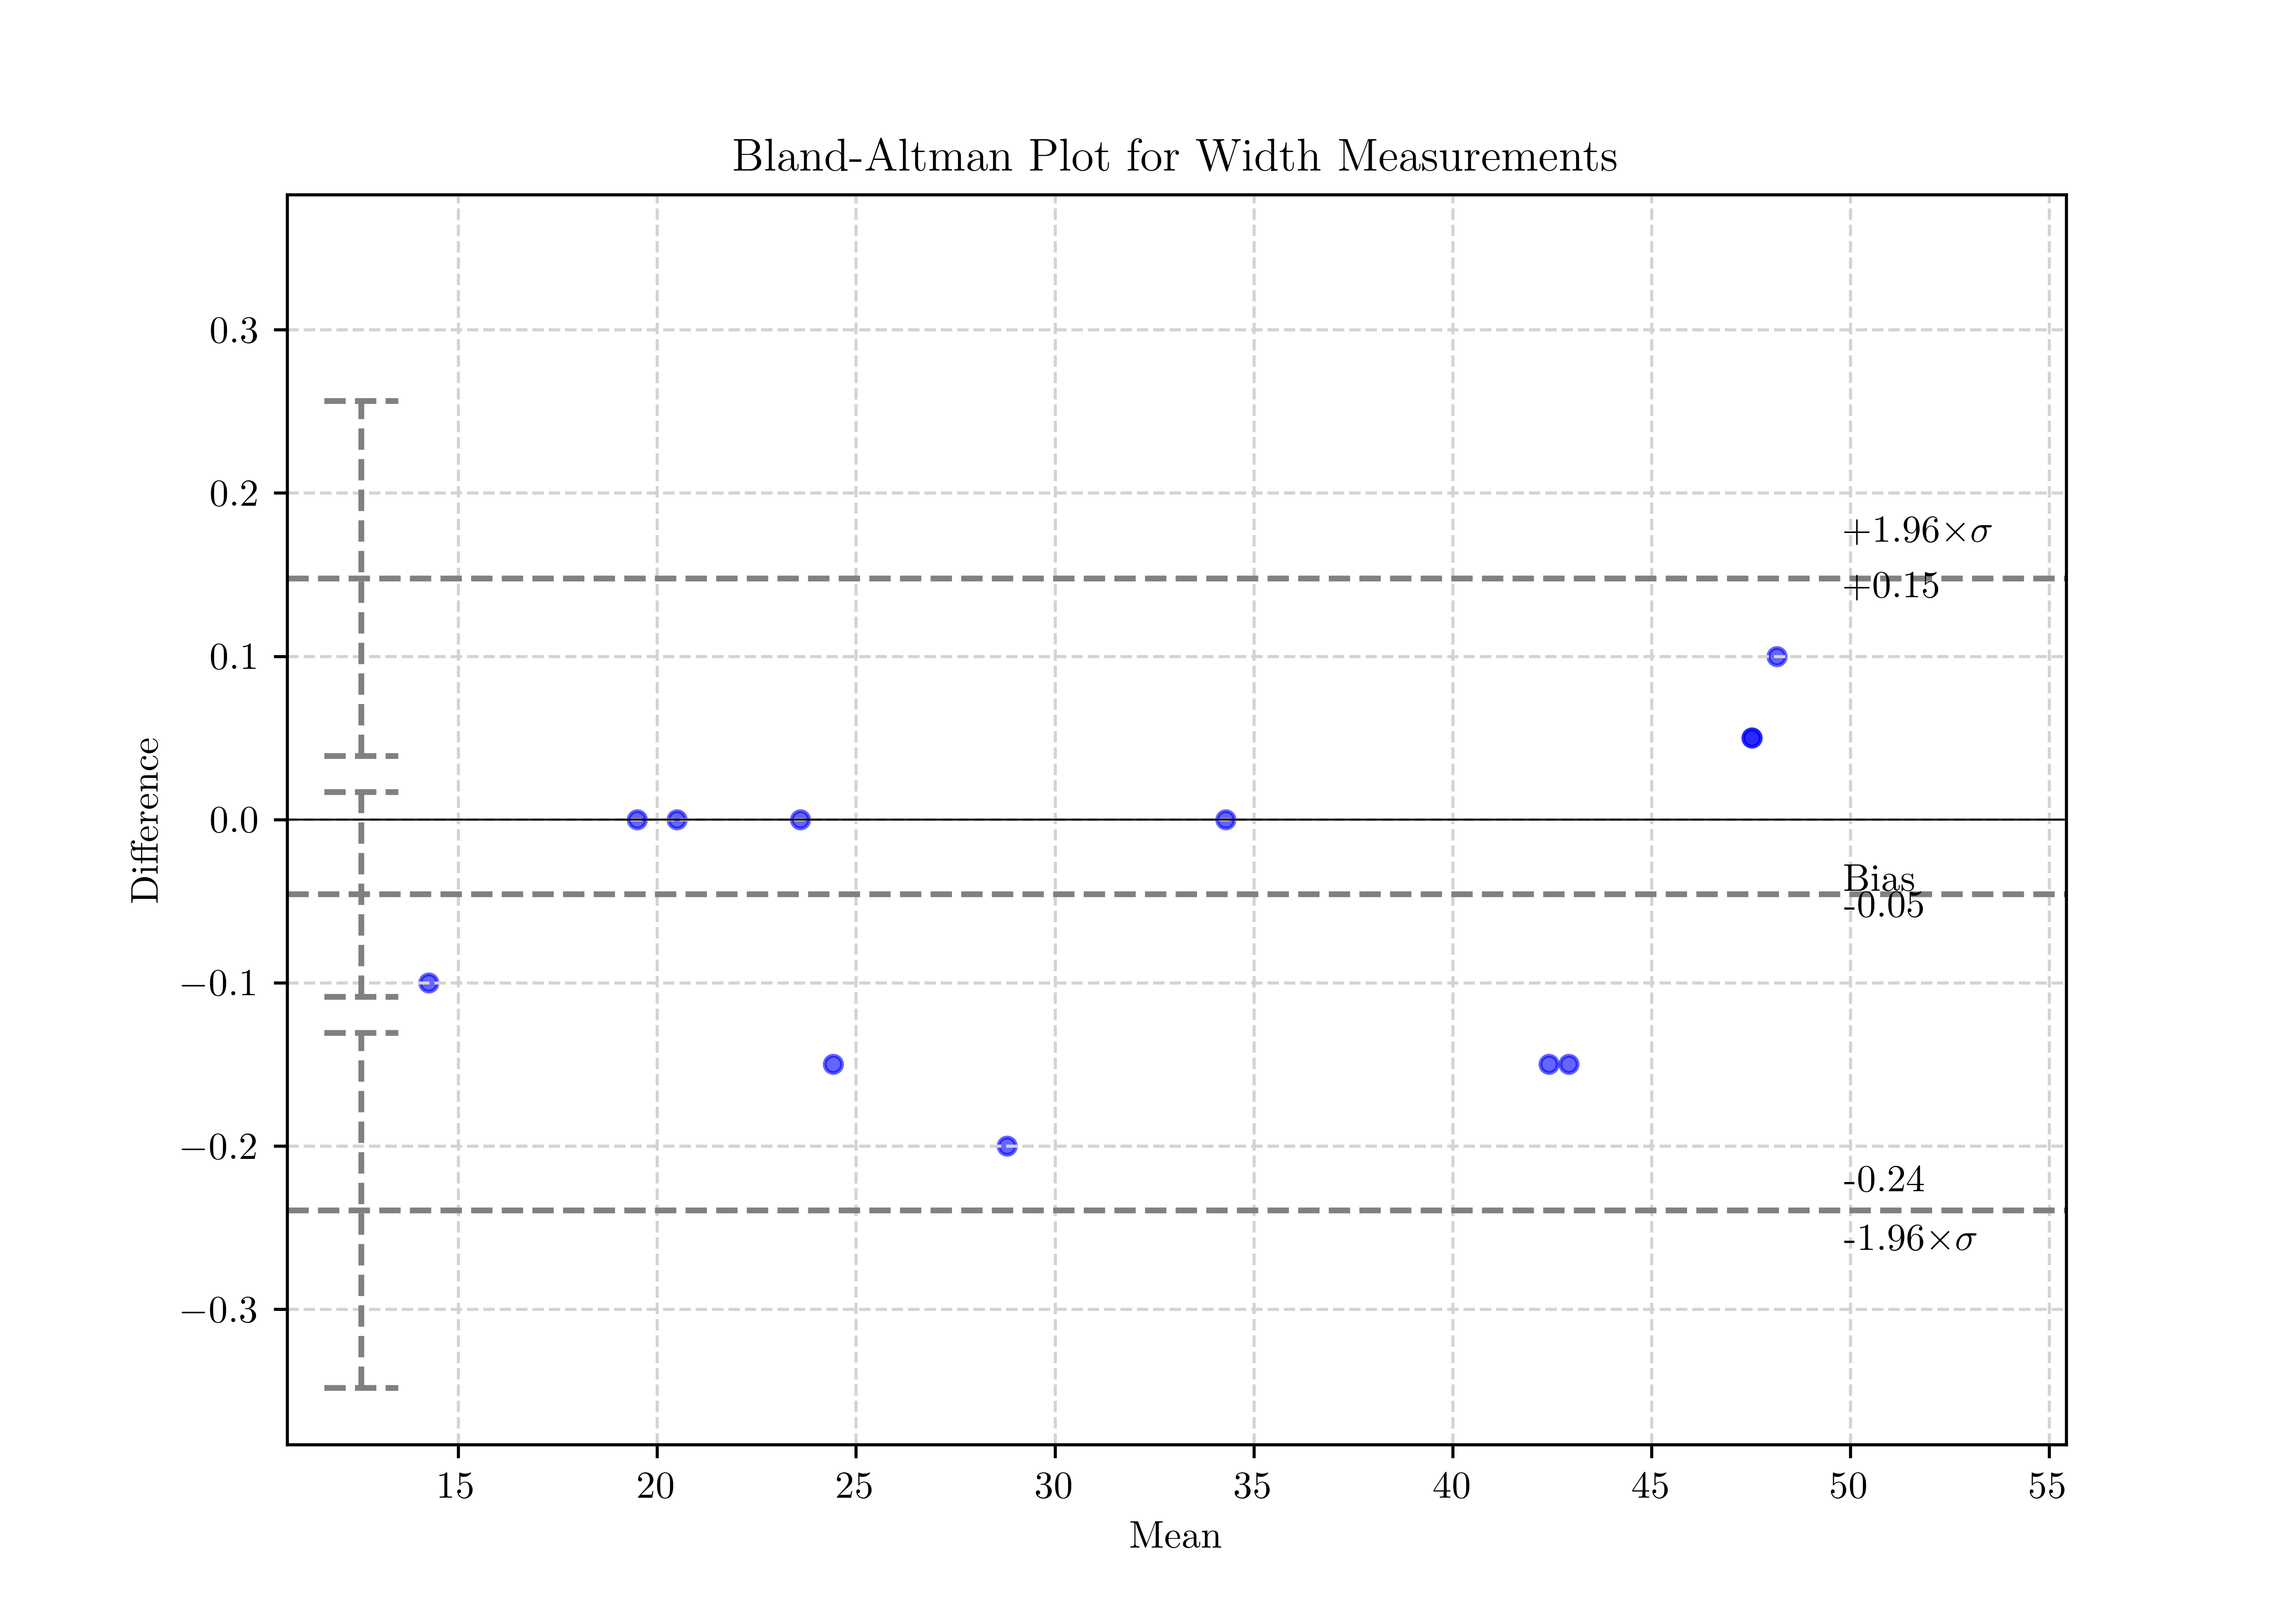
\includegraphics[width=0.75\linewidth]{images/chap5/width.png}
    \caption{Bland-Altman plot showcasing the width measurements obtained.}
    \label{fig:Bland-Altman_width}
\end{figure}


Another widely used tool to assess the relationship between two measurement methods is the Passing-Bablok method \autocite{Passing1983A}. This methodology of statistical analysis is especially useful when assessing agreement between methods without making assumptions about the linearity of the relationship or the presence of systematic errors in the reference data. Unlike linear regression, which assumes a linear relationship between the variables and the absence of systematic errors or assumes that there are errors following a normal distribution, the Passing-Bablok method can handle different forms of relationship between the variables and allows for the presence of systematic errors.

This statistical approach is particularly valuable when there is knowledge that there are systematic errors, such as comparing two measured data using different techniques. The Passing-Bablok method provides a robust assessment of agreement between measurement methods, even in the presence of systematic errors, and helps understand the relationship between the variables under study.

Figures \ref{fig:Passing-Bablok_height} and \ref{fig:Passing-Bablok_width} show a slope coefficient very close to one, indicating a strong correlation between the measurement systems with a small systematic error present. Additionally, it can be observed that the uncertainty remains constant throughout the sample group. This allows us to conclude that, for this group, there is a consistent tendency to preserve this correlation between the measurement methods.


\begin{figure}
    \centering
    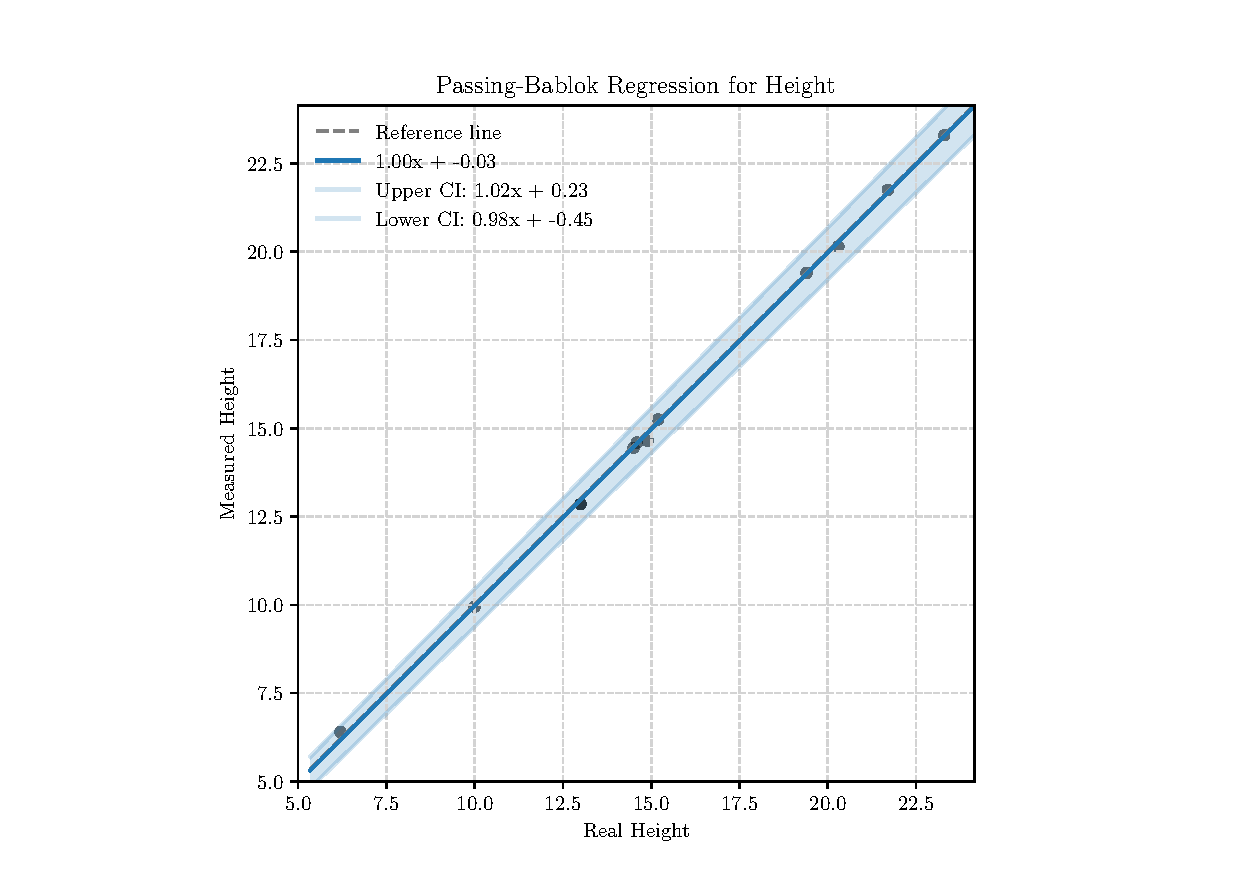
\includegraphics[width=0.75\linewidth]{images/chap5/Passing-Bablok_height.pdf}
    \caption{Passing-Bablok analysis obtained for height measurements. It can be observed the presence of a systematic error proportional to the measurement values. Additionally, a strong correlation between both measurement systems is evident.}
    \label{fig:Passing-Bablok_height}
\end{figure}

\begin{figure}
    \centering
    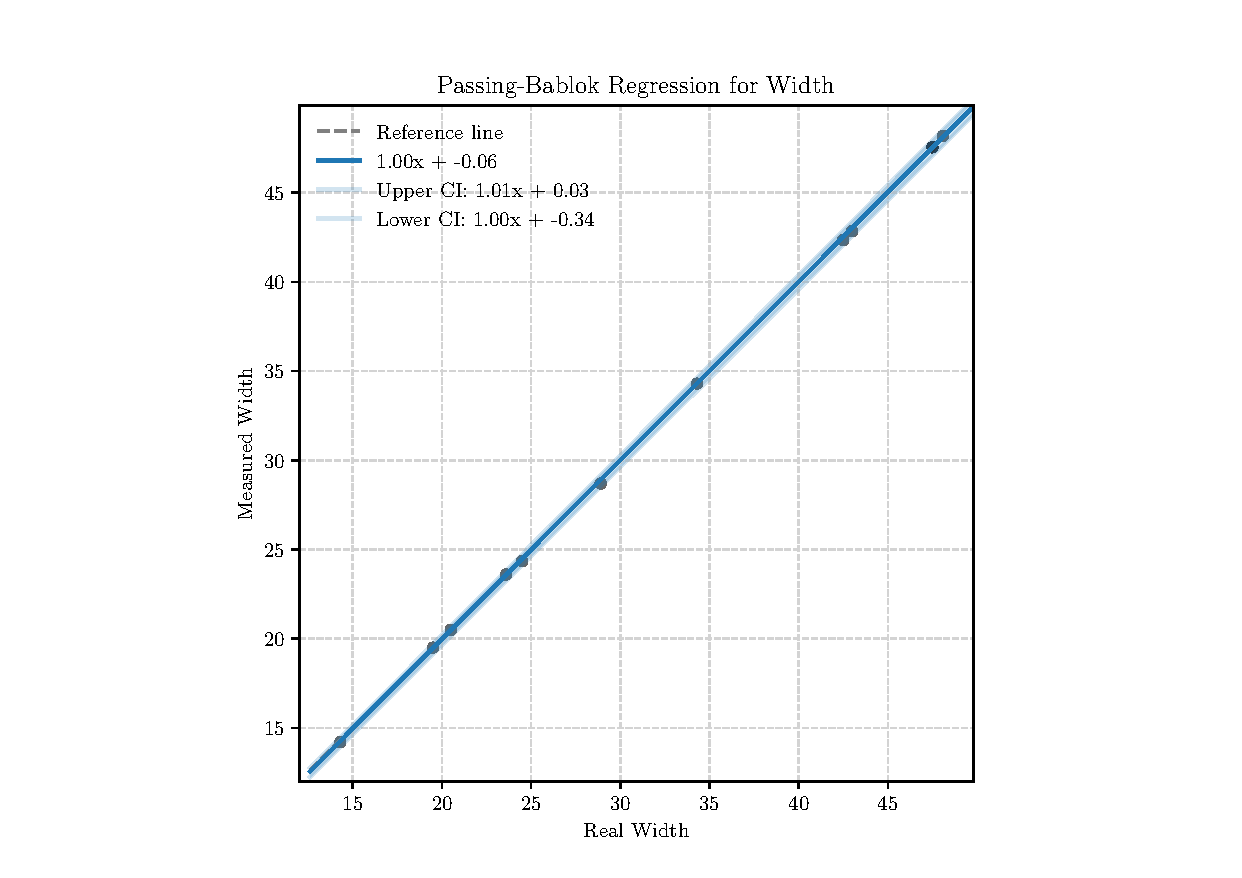
\includegraphics[width=0.75\linewidth]{images/chap5/Passing-Bablok_width.pdf}
    \caption{Passing-Bablok analysis obtained for width measurements. The presence of a systematic error proportional to the measured values can be observed, but the significance is lower than the values obtained for height. Furthermore, a strong correlation between the two measurement systems is evident.}
    \label{fig:Passing-Bablok_width}
\end{figure}


The graphs in Figures \ref{fig:Bland-Altman_height} and \ref{fig:Bland-Altman_width} reveal a systematic trend in height and width measurements, with a bias of -0.4 and -0.5, respectively. However, there is no evidence of anomalous behavior in the sample that indicates measurements outside the range of reliability. Therefore, we can conclude that there is a systematic error present, but the visual measurement instrument can be considered a viable option compared to the traditional method of measurement using a tape measure. Additionally, the graphs in Figures \ref{fig:Passing-Bablok_height} and \ref{fig:Passing-Bablok_width} show a strong correlation between both measurement systems, albeit with a small systematic error present. Thus, we can conclude that the proposed system can be used to replace the standard measurement system, taking into account the caveats regarding systematic errors, which can be improved in the future.


In efforts to estimate the inherent random uncertainties in the measurement process, a specific procedure was meticulously followed. A single wooden piece, with dimensions precisely measured to be 21.2 cm by 21 cm using a tape measure, served as the subject of this procedure. This chosen procedure is consistent with the methodology reported earlier for the statistical measurements. 

To capture measurements using a camera, a unique approach was taken to ensure a diverse data set. Specifically, the wooden piece was incrementally rotated approximately thirty degrees between each photograph. This process aimed to capture the possible variance in measurements due to different orientations. 

The comprehensive results of these measurement efforts are presented in the subsequent table.

\begin{table}[h]
\centering
\label{table:data}
\begin{tabular}{c c c c }
\hline
\textbf{Real Width} & \textbf{Real Height} & \textbf{Measured Width} & \textbf{Measured Height} \\
\hline
21.2 & 21 & 21.2 & 21 \\
21.2 & 21 & 21.3 & 21 \\
21.2 & 21 & 21.25 & 20.85 \\
21.2 & 21 & 21.2 & 20.85 \\
21.2 & 21 & 21.25 & 21 \\
21.2 & 21 & 21.2 & 21.05 \\
21.2 & 21 & 21.2 & 20.95 \\
21.2 & 21 & 21.45 & 21.15 \\
21.2 & 21 & 21.3 & 21.05 \\
21.2 & 21 & 21.4 & 21.65 \\
21.2 & 21 & 21.65 & 21.15 \\
21.2 & 21 & 21.3 & 21.25 \\
\hline
\end{tabular}
\caption{Width and Height Measurements for Normal Distribution}
\end{table}

When applying the given data to the Gaussian distribution equation (see Equation \ref{eq:gaussD}), one can generate the following chart \ref{fig:normal}:
\begin{figure}
    \centering
    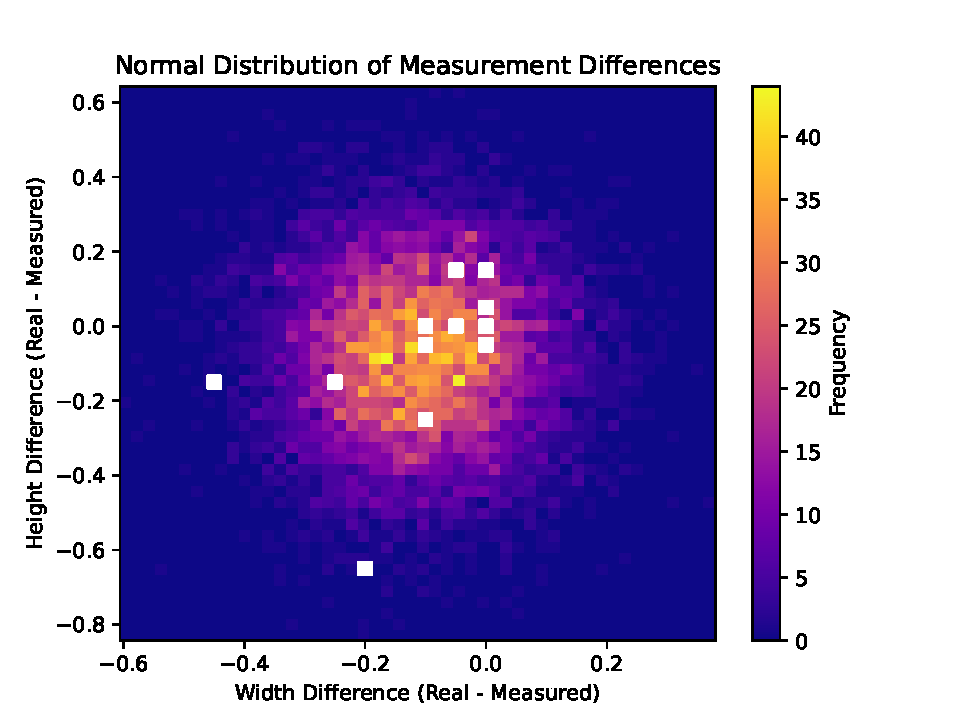
\includegraphics[width=0.65\linewidth]{images/chap5/Normal.pdf}
    \caption{Illustration of the Gaussian distribution obtained.}
    \label{fig:normal}
\end{figure}

\begin{equation}
f(x) = \frac{1}{\sigma\sqrt{2\pi}} e^{ -\frac{1}{2} \left( \frac{x-\mu}{\sigma} \right)^2 }
\label{eq:gaussD}
\end{equation}

In this equation: 
\begin{itemize}
\item \(f(x)\) is the probability density function
\item \(x\) is the variable
\item \(\mu\) is the mean or expectation of the distribution (and also its median and mode)
\item \(\sigma\) is the standard deviation
\item \(\sigma^2\) is the variance
\item \(e\) is the base of natural logarithms (approximately equal to 2.71828)
\item \(\pi\) is a mathematical constant whose approximate value is 3.14159
\end{itemize}

The standard deviation of the differences between the real and measured widths, denoted as $w$, was calculated to be approximately 0.1288. This value indicates that the differences between the real and measured widths are relatively close to the mean difference. This means that the measurements for width are generally quite accurate, with a small spread of error.

On the other hand, the standard deviation of the differences between the real and measured heights, denoted as $h$, was found to be approximately 0.2056. This value, being higher than the standard deviation for width, suggests that the measurements for height are more spread out from the mean difference. Therefore, the measurements for height display a larger spread of error compared to the measurements for width.

\newpage
\subsection{Ability to store leftover Data}
After detecting the characteristics of a leftover, they can be sent to the company's database or not. For this to occur, an entity must be created in the Orion-LD GE Context Broker. This creation only occurs if, after sending the image to the WW4 software, there is an attribute called "created" with the value "true". In this way, the API sends a signal to the Context Broker to create an entity of the "leftover" type in the company's storage system. Thus, the data is integrated into the system. The diagram in Figure \ref{fig:storage-diagram} illustrates this process well. Similarly, Figure \ref{fig:database-storage} shows the result of this process.

\begin{figure}[!ht]
    \centering
    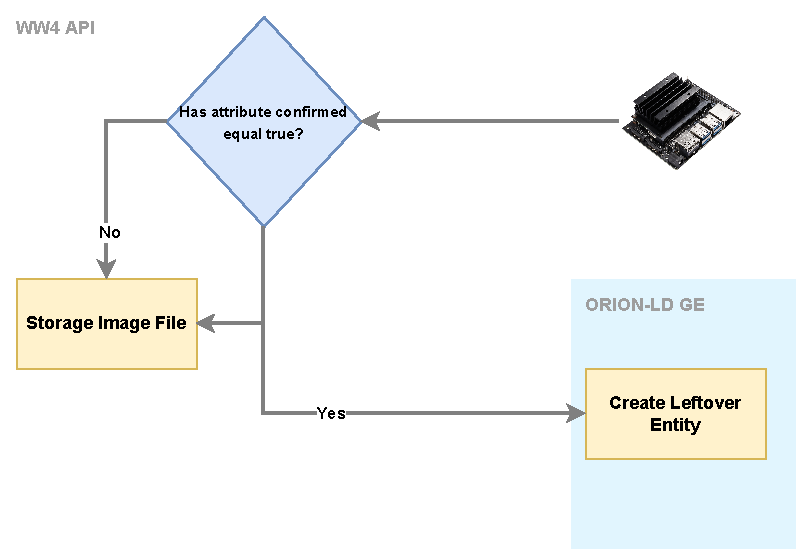
\includegraphics[width=0.65\linewidth]{images/chap5/Storage.pdf}
    \caption{Diagram illustrating the logical operation for adding a leftover to the company's data system.}
    \label{fig:database-diagram}
\end{figure}

Additionally, it is possible to attach a QR Code to the piece of wood, which will easily identify its characteristics, as exemplified by the QR Code below, generated for tracking a leftover piece that is stored in the database. When a user accesses it with the correct credentials, they can obtain relevant information about the wood piece. As can seen in the Figure \ref{fig:database-storage}.
\begin{figure}[H]
    \centering
    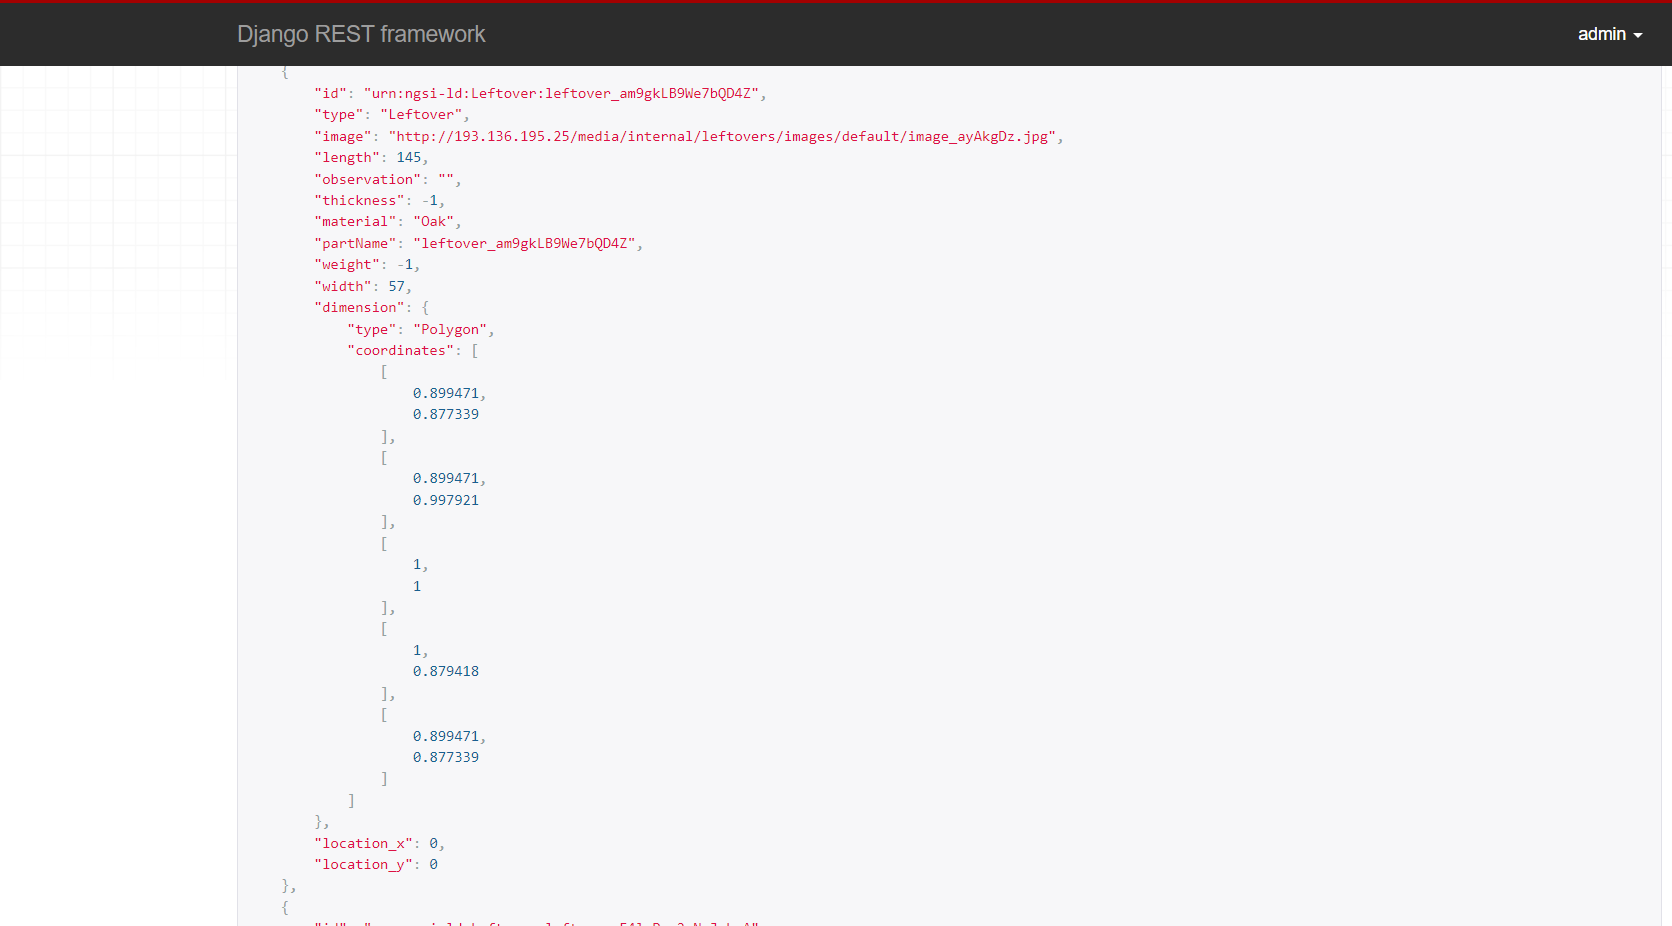
\includegraphics[width=0.65\linewidth]{images/chap5/leftover-storage.png}
    \caption{Result of a GET query showing the presence of leftovers in the company's database.}
    \label{fig:database-storage-qr}
\end{figure}



\begin{figure}[!ht]
    \centering
    
\includegraphics[width=0.35\linewidth]{images/chap5/adobe_express.png}
    \caption{Image of a QR code generated to facilitate easy tracking of the piece's information.}
    \label{fig:database-storage}
\end{figure}

\section{Article Publication}

A research paper was successfully accepted and published in a conference endorsed by IEEE, which took place in China. This was part of the effort to disseminate knowledge through academic articles. Additionally, another article was published in the SASYR (Symposium of Applied Science for Young Researchers). The citations for these papers can be found in Appendix \ref{apendice3}.
